\documentclass[aspectratio=169]{beamer}

% =================================================================
%  Basics of Automation and Control
%  A beginner-friendly Beamer deck (fully self-contained: all
%  figures / flowcharts / plots drawn with TikZ, so it compiles anywhere).
% =================================================================

% -------------------------------------------------
% Theme and packages
% -------------------------------------------------
\usetheme{Madrid}
\usecolortheme{default}

\usepackage{amsmath}
\usepackage{amssymb}
\usepackage{bm}
\usepackage{listings}
\usepackage{tikz}
\usepackage{array}
\usepackage{booktabs}
\usepackage{tabularx}
\usepackage{ragged2e}
\usepackage{xcolor}

\usetikzlibrary{shapes.geometric, arrows.meta, positioning, calc, fit, backgrounds}

% -------------------------------------------------
% Colour palette
% -------------------------------------------------
\definecolor{cAccent}{RGB}{0,102,153}     % teal-blue accent
\definecolor{cBox}{RGB}{28,31,42}          % dark box
\definecolor{cGreen}{RGB}{34,139,34}
\definecolor{cRed}{RGB}{178,34,34}
\definecolor{cOrange}{RGB}{204,102,0}
\definecolor{cPurple}{RGB}{102,45,145}
\definecolor{cGrayBg}{RGB}{245,246,248}
\definecolor{codebg}{RGB}{248,248,244}
\definecolor{codekw}{RGB}{0,0,180}
\definecolor{codecomment}{RGB}{0,130,0}
\definecolor{codestr}{RGB}{170,55,20}

% Beamer colour tweaks (match a Madrid-style accent)
\setbeamercolor{structure}{fg=cAccent}
\setbeamertemplate{frametitle continuation}{%
	\ifnum\insertcontinuationcount>1\space(cont...)\fi
}
\setbeamertemplate{navigation symbols}{}
\setbeamertemplate{caption}[numbered]

% -------------------------------------------------
% Listings style for C code
% -------------------------------------------------
\lstdefinestyle{cstyle}{
	language=C,
	backgroundcolor=\color{codebg},
	basicstyle=\ttfamily\footnotesize,
	keywordstyle=\color{codekw}\bfseries,
	commentstyle=\color{codecomment}\itshape,
	stringstyle=\color{codestr},
	numbers=none,
	numberstyle=\tiny\color{gray},
	numbersep=8pt,
	showstringspaces=false,
	breaklines=true,
	frame=single,
	rulecolor=\color{gray!50},
	tabsize=2,
	columns=fullflexible,
	keepspaces=true,
	literate={~}{{$\sim$}}1
}
\lstset{style=cstyle}

% Handy TikZ flowchart node styles
\tikzset{
	startstop/.style={rectangle, rounded corners=10pt, minimum width=2.4cm, minimum height=0.8cm, text centered, align=center, draw=black, fill=cAccent!25},
	process/.style  ={rectangle, minimum width=2.6cm, minimum height=0.8cm, text centered, align=center, text width=2.8cm, draw=black, fill=blue!8},
	io/.style       ={trapezium, trapezium left angle=70, trapezium right angle=110, minimum width=2.2cm, minimum height=0.8cm, text centered, align=center, draw=black, fill=cOrange!20},
	decision/.style ={diamond, aspect=2, minimum width=2.4cm, minimum height=0.9cm, text centered, text width=2.2cm, draw=black, fill=cGreen!18, inner sep=1pt},
	flowarrow/.style={-{Stealth[length=2.5mm]}, thick},
	% control-system block diagram styles
	blk/.style      ={rectangle, draw=black, thick, minimum width=1.9cm, minimum height=0.9cm, align=center, fill=blue!8},
	sumj/.style     ={circle, draw=black, thick, minimum size=0.55cm, inner sep=0pt},
	sig/.style      ={-{Stealth[length=2.2mm]}, thick},
	% valve / fluid-power symbols
	vflow/.style    ={-{Stealth[length=2mm]}, thick},
}

% -------------------------------------------------
% Small drawing helpers (valve and ladder symbols)
% -------------------------------------------------
% Spring (zig-zag) starting at point (#1,#2), drawn to the right
\newcommand{\vspring}[2]{%
	\draw[thick] (#1,#2) -- ++(0.08,0.18) -- ++(0.1,-0.36) -- ++(0.1,0.36) -- ++(0.1,-0.36) -- ++(0.1,0.36) -- ++(0.08,-0.18);}
% Solenoid (box with diagonal) ending at point (#1,#2), drawn to the left
\newcommand{\vsolenoid}[2]{%
	\draw[thick] ({#1-0.45},{#2-0.22}) rectangle (#1,{#2+0.22});
	\draw[thick] ({#1-0.45},{#2-0.22}) -- (#1,{#2+0.22});}
% Blocked port ("T" symbol) at bottom point (#1,#2), height #3 (negative = from top)
\newcommand{\vblock}[3]{%
	\draw[thick] (#1,#2) -- (#1,{#2+#3});
	\draw[thick] ({#1-0.12},{#2+#3}) -- ({#1+0.12},{#2+#3});}
% Ladder-logic symbols: normally-open / normally-closed contact and coil
\newcommand{\ladNO}[3]{%
	\draw[thick] ({#1-0.15},{#2-0.25}) -- ({#1-0.15},{#2+0.25});
	\draw[thick] ({#1+0.15},{#2-0.25}) -- ({#1+0.15},{#2+0.25});
	\node[above=1pt, font=\scriptsize] at (#1,{#2+0.25}) {#3};}
\newcommand{\ladNC}[3]{%
	\ladNO{#1}{#2}{#3}
	\draw[thick] ({#1-0.25},{#2-0.3}) -- ({#1+0.25},{#2+0.3});}
\newcommand{\ladCoil}[3]{%
	\draw[thick] (#1,#2) circle (0.28);
	\node[above=1pt, font=\scriptsize] at (#1,{#2+0.28}) {#3};}

\setbeamertemplate{footnote}{%
	\parindent 0em
	\noindent
	\raggedright
	\insertfootnotemark\insertfootnotetext\par
}

% -------------------------------------------------
% Title information
% -------------------------------------------------
\title[Basics of Automation \& Control]{Basics of Automation and Control}
\subtitle{Industrial Processes, Control Elements, Actuators \& PID}
\author[Amit Kumar Singh]{}
\institute[]{
	Amit Kumar Singh \\
	\vspace{0.1cm}
	Assistant Professor (ECE) \\
	\vspace{0.05cm}
	School of Naval Architecture and Ocean Engineering\\
	\vspace{0.05cm}
	Indian Maritime University Visakhapatnam Campus, Sabbavaram Mandal\\
	\vspace{0.05cm}
	Visakhapatnam, Andhra Pradesh -- 531~035\\
	\vspace{0.25cm}
	amitkumarsingh@imu.ac.in
}
\date[AI \& Automation]{\today}

\begin{document}

	%------------------------------------------------
	\begin{frame}
		\titlepage
	\end{frame}

	%------------------------------------------------
	\begin{frame}{Outline}
		\small
		\begin{columns}[T,onlytextwidth]
			\hspace{0.8cm}% shift the first column to the right
			\begin{column}{0.49\textwidth}
				\tableofcontents[hideallsubsections, sections={1-6}]
			\end{column}
			\hspace{0.8cm}% wider gap between the two columns
			\begin{column}{0.40\textwidth}
				\tableofcontents[hideallsubsections, sections={7-12}]
			\end{column}
		\end{columns}
	\end{frame}

	% =================================================================
	\section{Industrial Processes}
	% =================================================================
	\begin{frame}{What is an Industrial Process?}
		\begin{block}{Definition}
			An \textbf{industrial process} is a planned sequence of \textbf{physical}, \textbf{chemical},
			or \textbf{mechanical} operations that converts \textbf{raw materials} (input) into
			useful \textbf{products} (output) using energy, machines and people.
		\end{block}
		\vspace{0.3cm}
		\begin{columns}
			\begin{column}{0.58\textwidth}
				\begin{itemize}
					\item It follows the simple cycle:
					\[
					\textbf{RAW MATERIAL} \;\rightarrow\; \textbf{PROCESS} \;\rightarrow\; \textbf{PRODUCT}
					\]
					\item Examples: refining crude oil, generating power, bottling drinks, welding a ship hull.
					\item Every process has quantities that must be \emph{kept at the right value} ---
					temperature, pressure, flow, level, speed, position.
				\end{itemize}
			\end{column}
			\begin{column}{0.42\textwidth}
				\centering
				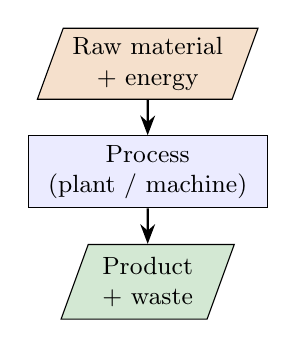
\begin{tikzpicture}[node distance=0.45cm, every node/.style={font=\small}]
					\node[io, fill=cOrange!20] (in) {Raw material\\ + energy};
					\node[process, below=of in] (proc) {Process\\ (plant / machine)};
					\node[io, below=of proc, fill=cGreen!20] (out) {Product\\ + waste};
					\draw[flowarrow] (in) -- (proc);
					\draw[flowarrow] (proc) -- (out);
				\end{tikzpicture}
			\end{column}
		\end{columns}
	\end{frame}

	\begin{frame}{Types of Industrial Processes}
		\begin{columns}[T]
			\begin{column}{0.32\textwidth}
				\begin{block}{Continuous}
					\centering
					\textbf{Runs non-stop, 24 $\times$ 7}

					\vspace{0.2cm}

					\begin{itemize}\small
						\item Material flows without interruption.
						\item Variables are \emph{analog} (temperature, flow, level).
						\item Examples: oil refinery, power plant, water treatment.
					\end{itemize}
				\end{block}
			\end{column}
			\begin{column}{0.32\textwidth}
				\begin{block}{Batch}
					\centering
					\textbf{Fixed quantity at a time}

					\vspace{0.2cm}

					\begin{itemize}\small
						\item A recipe is run step by step on one lot.
						\item Mix $\rightarrow$ heat $\rightarrow$ hold $\rightarrow$ empty.
						\item Examples: medicines, paint, food, beverages.
					\end{itemize}
				\end{block}
			\end{column}
			\begin{column}{0.32\textwidth}
				\begin{block}{Discrete}
					\centering
					\textbf{Individual countable parts}

					\vspace{0.2cm}

					\begin{itemize}\small
						\item Parts are made, moved and assembled.
						\item Variables are mostly \emph{ON/OFF} (part present, cylinder out).
						\item Examples: car assembly, packaging, shipbuilding.
					\end{itemize}
				\end{block}
			\end{column}
		\end{columns}
		\vspace{0.35cm}
		\begin{center}
			\small
			Continuous \& batch $\rightarrow$ mainly \textbf{process control} (PID loops)\\
			Discrete $\rightarrow$ mainly \textbf{sequence / logic control} (PLC)
		\end{center}
	\end{frame}

	\begin{frame}{Process Variables and Signals}
		\renewcommand{\arraystretch}{1.3}
		\centering
		\begin{tabular}{@{}llll@{}}
			\toprule
			\textbf{Variable} & \textbf{Unit} & \textbf{Typical sensor} & \textbf{Example} \\
			\midrule
			Temperature & $^\circ$C, K     & Thermocouple, RTD (Pt100)          & boiler, engine cooling \\
			Pressure    & bar, Pa          & Strain-gauge / piezo transmitter   & steam line, hydraulics \\
			Flow        & m$^3$/h, L/min   & Orifice + DP cell, magnetic meter  & fuel, cooling water \\
			Level       & m, \%            & Float, ultrasonic, DP transmitter  & ballast tank, boiler drum \\
			Speed / position & rpm, mm     & Tachogenerator, encoder, LVDT      & shaft, rudder angle \\
			\bottomrule
		\end{tabular}
		\vspace{0.3cm}
		\begin{columns}[T]
			\begin{column}{0.5\textwidth}
				\begin{block}{Standard instrument signals}
					\small
					\textbf{4--20 mA} (current loop), \textbf{0--10 V}, pneumatic \textbf{0.2--1.0 bar} (3--15 psi).
				\end{block}
			\end{column}
			\begin{column}{0.5\textwidth}
				\begin{block}{Why 4 mA and not 0 mA?}
					\small A ``live zero'': 0 mA means a \textbf{broken wire}, not a zero reading.
				\end{block}
			\end{column}
		\end{columns}
	\end{frame}

	\begin{frame}{Converting a 4--20 mA Signal: Worked Example}
		\begin{block}{Linear scaling}
			\[
			\text{PV} \;=\; \text{LRV} + \frac{I - 4}{20 - 4}\times(\text{URV} - \text{LRV})
			\]
			LRV / URV = lower / upper range value of the transmitter.
		\end{block}
		\vspace{0.1cm}
		\begin{columns}[T]
			\begin{column}{0.5\textwidth}
				\textbf{Problem:} a temperature transmitter is ranged 0--200\,$^\circ$C.
				The controller reads \textbf{12 mA}. What is the temperature?
				\vspace{0.2cm}

				\textbf{Solution:}
				\[
				T = 0 + \frac{12-4}{16}\times 200 = \frac{8}{16}\times 200 = \boxed{100\,^\circ\text{C}}
				\]
			\end{column}
			\begin{column}{0.5\textwidth}
				\centering
				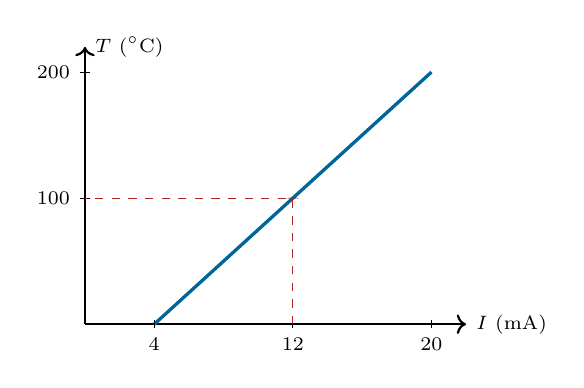
\begin{tikzpicture}[font=\scriptsize, x=0.22cm, y=0.016cm]
					\draw[->, thick] (0,0) -- (22,0) node[right] {$I$ (mA)};
					\draw[->, thick] (0,0) -- (0,220) node[right] {$T$ ($^\circ$C)};
					\draw[very thick, cAccent] (4,0) -- (20,200);
					\foreach \x in {4,12,20} \draw (\x,3) -- (\x,-3) node[below] {\x};
					\foreach \y in {100,200} \draw (0.3,\y) -- (-0.3,\y) node[left] {\y};
					\draw[dashed, cRed] (12,0) -- (12,100) -- (0,100);
					\fill[cRed] (12,100) circle (0.35);
				\end{tikzpicture}
			\end{column}
		\end{columns}
	\end{frame}

	% =================================================================
	\section{Automation of Industrial Processes}
	% =================================================================
	\begin{frame}{What is Automation?}
		\begin{block}{Automation}
			\textbf{Automation} is the use of \textbf{control systems} (sensors, controllers,
			actuators, computers) to operate machines and processes with \textbf{minimum human intervention}.
		\end{block}
		\vspace{0.2cm}
		\begin{columns}[T]
			\begin{column}{0.5\textwidth}
				\begin{block}{Why automate?}
					\begin{itemize}\small
						\item Higher \textbf{productivity} and consistent \textbf{quality}.
						\item \textbf{Safety} --- remove people from hazardous areas.
						\item Lower operating cost, less waste \& energy.
						\item Accurate data logging and remote monitoring.
					\end{itemize}
				\end{block}
			\end{column}
			\begin{column}{0.5\textwidth}
				\begin{block}{Limitations}
					\begin{itemize}\small
						\item High initial (capital) cost.
						\item Needs skilled maintenance staff.
						\item Less flexible for one-off jobs.
						\item Cyber-security \& single-point failures.
					\end{itemize}
				\end{block}
			\end{column}
		\end{columns}
		\vspace{0.2cm}
		\footnotesize\centering
		On a ship: engine-room automation lets an \emph{unmanned machinery space} (UMS) run safely at night.
	\end{frame}

	\begin{frame}{Types of Automation}
		\renewcommand{\arraystretch}{1.4}
		\centering
		\begin{tabular}{@{}>{\raggedright}p{2.5cm}>{\raggedright}p{3.9cm}>{\raggedright}p{3.0cm}>{\raggedright\arraybackslash}p{3.2cm}@{}}
			\toprule
			\textbf{Type} & \textbf{Idea} & \textbf{Volume / variety} & \textbf{Example} \\
			\midrule
			\textbf{Fixed} (hard)   & Sequence fixed by the equipment design & very high volume, one product & bottling line, transfer machine \\
			\textbf{Programmable}   & Sequence changed by a new program       & medium volume, batches        & CNC machine, PLC-driven press \\
			\textbf{Flexible}       & Changes product with no lost time       & medium volume, many variants  & robotic welding cell, FMS \\
			\bottomrule
		\end{tabular}
		\vspace{0.4cm}
		\begin{block}{Key idea}
			Moving down the table, the system becomes \textbf{more adaptable} but also \textbf{more complex} and costly per unit. The choice depends on \emph{how many} and \emph{how many different} products we make.
		\end{block}
	\end{frame}

	\begin{frame}{The Automation Pyramid (Levels of Control)}
		\begin{columns}[T]
			\begin{column}{0.58\textwidth}
				\centering
				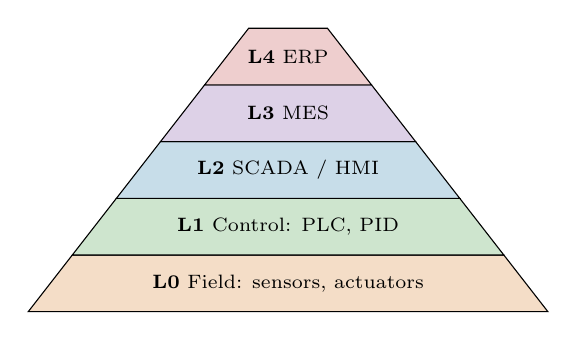
\begin{tikzpicture}[font=\scriptsize]
					\def\h{0.72}
					\foreach \i/\lab/\col in {
						0/{\textbf{L0} Field: sensors, actuators}/cOrange,
						1/{\textbf{L1} Control: PLC, PID}/cGreen,
						2/{\textbf{L2} SCADA / HMI}/cAccent,
						3/{\textbf{L3} MES}/cPurple,
						4/{\textbf{L4} ERP}/cRed} {
						\pgfmathsetmacro{\yb}{\i*\h}
						\pgfmathsetmacro{\yt}{(\i+1)*\h}
						\pgfmathsetmacro{\wb}{3.3-0.56*\i}
						\pgfmathsetmacro{\wt}{3.3-0.56*(\i+1)}
						\filldraw[draw=black, fill=\col!22] (-\wb,\yb) -- (\wb,\yb) -- (\wt,\yt) -- (-\wt,\yt) -- cycle;
						\node at (0,{(\i+0.5)*\h}) {\lab};
					}
				\end{tikzpicture}

				\vspace{0.1cm}
				\footnotesize Going \textbf{up}: slower, more data, business view.\\
				Going \textbf{down}: faster, real-time, closer to the machine.
			\end{column}
			\begin{column}{0.42\textwidth}
				\begin{itemize}\small
					\item \textbf{Field}: measure and act on the process (ms).
					\item \textbf{Control}: run the control logic / loops (ms--s).
					\item \textbf{Supervisory}: operator screens, alarms, trends (s).
					\item \textbf{MES / ERP}: production planning, orders, business (hours--days).
				\end{itemize}
				\vspace{0.2cm}
				\footnotesize This course concentrates on \textbf{Levels 0 and 1}.
			\end{column}
		\end{columns}
	\end{frame}

	\begin{frame}{Open-Loop vs.\ Closed-Loop Control}
		\vspace*{-0.2cm}
		\begin{block}{Open loop}
			\small Output is \textbf{not} measured --- the controller acts blindly (e.g.\ a toaster timer, a washing-machine cycle).
		\end{block}
		\centering
		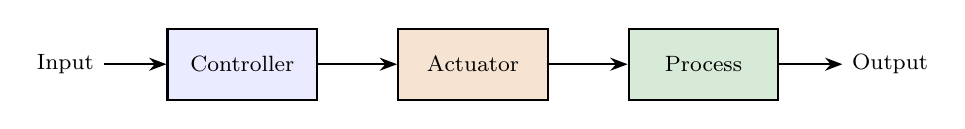
\begin{tikzpicture}[font=\footnotesize, node distance=1.0cm]
			\node (r) {Input};
			\node[blk, right=0.8cm of r] (c) {Controller};
			\node[blk, right=of c, fill=cOrange!18] (a) {Actuator};
			\node[blk, right=of a, fill=cGreen!18] (p) {Process};
			\node[right=0.8cm of p] (y) {Output};
			\draw[sig] (r) -- (c); \draw[sig] (c) -- (a); \draw[sig] (a) -- (p); \draw[sig] (p) -- (y);
		\end{tikzpicture}
		\begin{block}{Closed loop (feedback)}
			\small Output is \textbf{measured} and compared with the desired value; the \textbf{error} drives the controller (e.g.\ AC thermostat, autopilot).
		\end{block}
		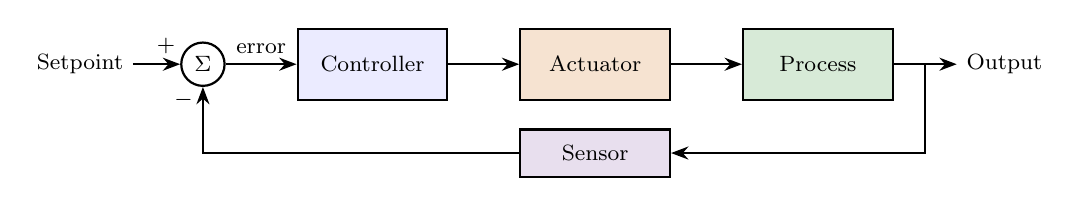
\begin{tikzpicture}[font=\footnotesize, node distance=0.9cm]
			\node (r) {Setpoint};
			\node[sumj, right=0.6cm of r] (s) {$\Sigma$};
			\node[blk, right=of s] (c) {Controller};
			\node[blk, right=of c, fill=cOrange!18] (a) {Actuator};
			\node[blk, right=of a, fill=cGreen!18] (p) {Process};
			\node[right=0.8cm of p] (y) {Output};
			\node[blk, below=0.35cm of a, fill=cPurple!15, minimum height=0.6cm] (m) {Sensor};
			\draw[sig] (r) -- node[above, pos=0.7] {$+$} (s);
			\draw[sig] (s) -- node[above] {error} (c);
			\draw[sig] (c) -- (a); \draw[sig] (a) -- (p);
			\draw[sig] (p) -- coordinate[pos=0.5] (tap) (y);
			\draw[sig] (tap) |- (m);
			\draw[sig] (m) -| node[left, pos=0.9] {$-$} (s);
		\end{tikzpicture}
	\end{frame}

	\begin{frame}{A Closed-Loop Example: Tank Level Control}
		\begin{columns}[T]
			\begin{column}{0.5\textwidth}
				\centering
				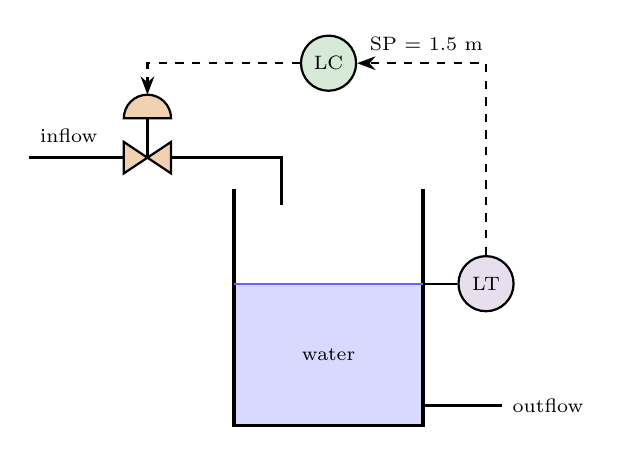
\begin{tikzpicture}[font=\scriptsize]
					% tank
					\fill[blue!15] (0,0) rectangle (2.4,1.8);
					\draw[very thick] (0,3) -- (0,0) -- (2.4,0) -- (2.4,3);
					\draw[blue!60, thick] (0,1.8) -- (2.4,1.8);
					\node at (1.2,0.9) {water};
					% inlet pipe with valve
					\draw[very thick] (-2.6,3.4) -- (-1.4,3.4);
					\draw[very thick] (-0.8,3.4) -- (0.6,3.4) -- (0.6,2.8);
					\filldraw[fill=cOrange!30, thick] (-1.4,3.2) -- (-1.4,3.6) -- (-0.8,3.2) -- (-0.8,3.6) -- cycle;
					\draw[thick] (-1.1,3.4) -- (-1.1,3.9);
					\draw[thick, fill=cOrange!30] (-1.4,3.9) arc (180:0:0.3) -- cycle;
					\node[above=2pt] at (-2.1,3.4) {inflow};
					% outlet
					\draw[very thick] (2.4,0.25) -- (3.4,0.25) node[right] {outflow};
					% level transmitter and controller
					\node[circle, draw, thick, fill=cPurple!15, minimum size=0.7cm, inner sep=0pt] (lt) at (3.2,1.8) {LT};
					\draw[thick] (2.4,1.8) -- (lt);
					\node[circle, draw, thick, fill=cGreen!18, minimum size=0.7cm, inner sep=0pt] (lc) at (1.2,4.6) {LC};
					\draw[dashed, thick, -{Stealth}] (lt) |- (lc);
					\draw[dashed, thick, -{Stealth}] (lc) -| (-1.1,4.2);
					\node[right] at (1.6,4.85) {SP = 1.5 m};
				\end{tikzpicture}
			\end{column}
			\begin{column}{0.5\textwidth}
				\begin{enumerate}\small
					\item \textbf{LT} (level transmitter) measures the level and sends 4--20 mA.
					\item \textbf{LC} (level controller) compares it with the \textbf{setpoint}.
					\item If the level is low, LC \textbf{opens} the inlet control valve more; if high, it \textbf{closes} it.
					\item The loop repeats continuously --- level stays at 1.5 m even if outflow changes (\emph{disturbance}).
				\end{enumerate}
				\vspace{0.2cm}
				\footnotesize Dashed lines = instrument signals; solid lines = process pipes (ISA-5.1 style).
			\end{column}
		\end{columns}
	\end{frame}

	% =================================================================
	\section{Elements of a Control System}
	% =================================================================
	\begin{frame}{Building Blocks of Every Control Loop}
		\centering
		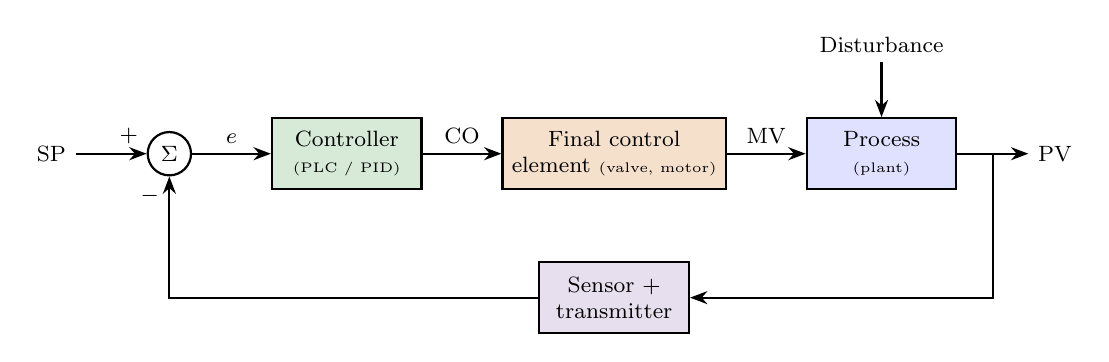
\begin{tikzpicture}[font=\footnotesize, node distance=1.0cm]
			\node[sumj] (s) {$\Sigma$};
			\node[left=0.9cm of s] (r) {SP};
			\node[blk, right=of s, fill=cGreen!18] (c) {Controller\\ \tiny(PLC / PID)};
			\node[blk, right=of c, fill=cOrange!20] (f) {Final control\\ element \tiny(valve, motor)};
			\node[blk, right=of f, fill=blue!12] (p) {Process\\ \tiny(plant)};
			\node[right=0.9cm of p] (y) {PV};
			\node[blk, below=0.9cm of f, fill=cPurple!15] (m) {Sensor +\\ transmitter};
			\node[above=0.7cm of p] (d) {Disturbance};
			\draw[sig] (r) -- node[above, pos=0.75] {$+$} (s);
			\draw[sig] (s) -- node[above] {$e$} (c);
			\draw[sig] (c) -- node[above] {CO} (f);
			\draw[sig] (f) -- node[above] {MV} (p);
			\draw[sig] (p) -- coordinate[pos=0.5] (tap) (y);
			\draw[sig] (d) -- (p);
			\draw[sig] (tap) |- (m);
			\draw[sig] (m) -| node[left, pos=0.92] {$-$} (s);
		\end{tikzpicture}
		\vspace{0.3cm}
		\renewcommand{\arraystretch}{1.15}
		{\small
			\begin{tabular}{@{}ll@{\qquad}ll@{}}
				\toprule
				\textbf{SP} & Setpoint (desired value) & \textbf{CO} & Controller output \\
				\textbf{PV} & Process variable (measured) & \textbf{MV} & Manipulated variable \\
				$\bm{e}$ & Error $= \text{SP} - \text{PV}$ & & (e.g.\ flow through valve) \\
				\bottomrule
		\end{tabular}}
	\end{frame}

	\begin{frame}{Three Families of Control Systems}
		\begin{columns}[T]
			\begin{column}{0.32\textwidth}
				\begin{block}{Pneumatic}
					\centering
					\textbf{Medium: compressed air}

					\vspace{0.2cm}

					\begin{itemize}\small
						\item 6--8 bar working pressure.
						\item Fast, clean, cheap, spark-free.
						\item Light loads, simple motion.
					\end{itemize}
				\end{block}
			\end{column}
			\begin{column}{0.32\textwidth}
				\begin{block}{Hydraulic}
					\centering
					\textbf{Medium: pressurised oil}

					\vspace{0.2cm}

					\begin{itemize}\small
						\item 100--350 bar working pressure.
						\item Very large forces, stiff \& precise.
						\item Steering gear, cranes, presses.
					\end{itemize}
				\end{block}
			\end{column}
			\begin{column}{0.32\textwidth}
				\begin{block}{Electrical}
					\centering
					\textbf{Medium: electric current}

					\vspace{0.2cm}

					\begin{itemize}\small
						\item Relays, contactors, PLCs, drives.
						\item Easy to transmit \& to program.
						\item Motors, solenoids, heaters.
					\end{itemize}
				\end{block}
			\end{column}
		\end{columns}
		\vspace{0.35cm}
		\begin{center}
			\small
			Modern machines are usually \textbf{electro-pneumatic} or \textbf{electro-hydraulic}:\\
			\textbf{electrical} signals decide, \textbf{fluid} power does the heavy work.
		\end{center}
	\end{frame}

	\begin{frame}{Comparing Pneumatic, Hydraulic \& Electrical Systems}
		\renewcommand{\arraystretch}{1.12}
		\centering
		\small
		\begin{tabular}{@{}>{\raggedright}p{2.8cm}>{\raggedright}p{3.4cm}>{\raggedright}p{3.4cm}>{\raggedright\arraybackslash}p{3.4cm}@{}}
			\toprule
			\textbf{Feature} & \textbf{Pneumatic} & \textbf{Hydraulic} & \textbf{Electrical} \\
			\midrule
			Force            & low--medium             & very high               & low--high \\
			Speed            & high                    & medium                  & high \\
			Position accuracy& poor (air compresses)   & good (oil is stiff)     & excellent (servo/stepper) \\
			Overload         & safe --- just stalls    & safe with relief valve  & needs protection \\
			Cleanliness      & clean, exhaust to air   & leaks are messy, fire risk & clean \\
			Cost             & low                     & high                    & medium \\
			Typical use      & packaging, clamping     & steering gear, presses  & conveyors, robots, pumps \\
			\bottomrule
		\end{tabular}
		\vspace{0.1cm}
		\begin{block}{Rule of thumb}
			\small \textbf{Big force}? $\rightarrow$ hydraulics. \quad \textbf{Fast, light, cheap}? $\rightarrow$ pneumatics. \quad \textbf{Precision}? $\rightarrow$ electrical.
		\end{block}
	\end{frame}

	% =================================================================
	\section{Pneumatic Control Systems}
	% =================================================================
	\begin{frame}{Elements of a Pneumatic System}
		\centering
		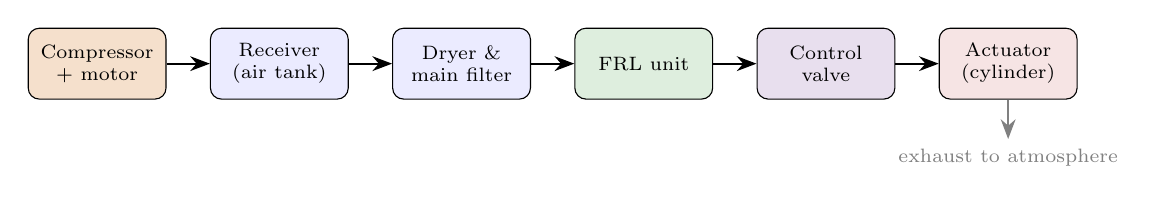
\begin{tikzpicture}[every node/.style={font=\scriptsize},
			el/.style={rectangle, draw=black, rounded corners, minimum width=1.75cm, minimum height=0.9cm, align=center, fill=blue!8}]
			\node[el, fill=cOrange!20] (comp) {Compressor\\ + motor};
			\node[el, right=0.55cm of comp] (rec) {Receiver\\ (air tank)};
			\node[el, right=0.55cm of rec] (dry) {Dryer \&\\ main filter};
			\node[el, right=0.55cm of dry, fill=cGreen!15] (frl) {FRL unit};
			\node[el, right=0.55cm of frl, fill=cPurple!15] (dcv) {Control\\ valve};
			\node[el, right=0.55cm of dcv, fill=cRed!12] (act) {Actuator\\ (cylinder)};
			\draw[flowarrow] (comp) -- (rec);
			\draw[flowarrow] (rec) -- (dry);
			\draw[flowarrow] (dry) -- (frl);
			\draw[flowarrow] (frl) -- (dcv);
			\draw[flowarrow] (dcv) -- (act);
			\draw[flowarrow, gray] (act.south) -- ++(0,-0.5) node[below] {exhaust to atmosphere};
		\end{tikzpicture}
		\vspace{0.3cm}
		\begin{itemize}\small
			\item \textbf{Compressor} --- raises air to 6--10 bar; \textbf{receiver} stores it and smooths pulsations.
			\item \textbf{Dryer / filter} --- removes water and dirt (moisture causes corrosion \& valve sticking).
			\item \textbf{FRL} = \textbf{F}ilter + \textbf{R}egulator (sets constant pressure) + \textbf{L}ubricator (oil mist).
			\item \textbf{Control valves} --- decide \emph{where}, \emph{how much} and \emph{how fast} air flows.
			\item \textbf{Actuators} --- turn air pressure into motion (cylinders, air motors).
		\end{itemize}
	\end{frame}

	\begin{frame}{Pneumatics: Properties of Compressed Air}
		\begin{columns}[T]
			\begin{column}{0.5\textwidth}
				\begin{block}{Advantages}
					\begin{itemize}\small
						\item Air is free and available everywhere.
						\item Easily stored and piped over distance.
						\item Explosion-proof --- no sparks (paint shops, mines, tankers).
						\item Actuators can stall under overload without damage.
						\item Very high speeds (up to 1--2 m/s for cylinders).
					\end{itemize}
				\end{block}
			\end{column}
			\begin{column}{0.5\textwidth}
				\begin{block}{Disadvantages}
					\begin{itemize}\small
						\item Air is \textbf{compressible} $\rightarrow$ uneven, ``spongy'' motion.
						\item Force limited (practical limit $\approx$ 30 kN).
						\item Exhaust noise --- silencers needed.
						\item Energy-inefficient (compressor losses, leaks).
						\item Air must be clean and dry.
					\end{itemize}
				\end{block}
			\end{column}
		\end{columns}
		\vspace{0.3cm}
		\begin{block}{Units to remember}
			\centering\small
			1 bar $= 10^5$ Pa $= 0.1$ MPa $\approx 14.5$ psi \qquad
			1 MPa $=$ 1 N/mm$^2$ \qquad Gauge pressure $=$ absolute $-$ atmospheric
		\end{block}
	\end{frame}

	\begin{frame}{Example Pneumatic Circuit: Double-Acting Cylinder}
		\begin{columns}[T]
			\begin{column}{0.5\textwidth}
				\centering
				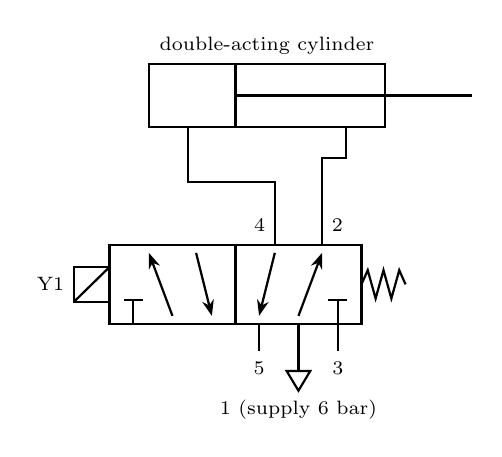
\begin{tikzpicture}[font=\scriptsize]
					% ---------- cylinder ----------
					\draw[thick] (0.5,2.5) rectangle (3.5,3.3);
					\draw[very thick] (1.6,2.5) -- (1.6,3.3);
					\draw[very thick] (1.6,2.9) -- (4.6,2.9);
					\node[above] at (2.0,3.3) {double-acting cylinder};
					% ---------- 5/2 valve (two boxes) ----------
					\draw[thick] (0,0) rectangle (1.6,1);
					\draw[thick] (1.6,0) rectangle (3.2,1);
					% actuated box (left): 1->4, 2->3, 5 blocked
					\draw[vflow] (0.8,0.1) -- (0.5,0.9);
					\draw[vflow] (1.1,0.9) -- (1.3,0.1);
					\vblock{0.3}{0}{0.3}
					% rest box (right): 1->2, 4->5, 3 blocked
					\draw[vflow] (2.4,0.1) -- (2.7,0.9);
					\draw[vflow] (2.1,0.9) -- (1.9,0.1);
					\vblock{2.9}{0}{0.3}
					% operators
					\vsolenoid{0}{0.5}
					\node[left] at (-0.45,0.5) {Y1};
					\vspring{3.2}{0.5}
					% ports of rest box
					\draw[thick] (1.9,0) -- (1.9,-0.35) node[below] {5};
					\draw[thick] (2.4,0) -- (2.4,-0.6);
					\draw[thick] (2.9,0) -- (2.9,-0.35) node[below] {3};
					\filldraw[fill=white, thick] (2.25,-0.6) -- (2.55,-0.6) -- (2.4,-0.85) -- cycle;
					\node[below] at (2.4,-0.85) {1 (supply 6 bar)};
					% lines to cylinder
					\draw[thick] (2.1,1) -- (2.1,1.8) -- (1.0,1.8) -- (1.0,2.5);
					\draw[thick] (2.7,1) -- (2.7,2.1) -- (3.0,2.1) -- (3.0,2.5);
					\node[left] at (2.1,1.25) {4};
					\node[right] at (2.7,1.25) {2};
				\end{tikzpicture}
			\end{column}
			\begin{column}{0.5\textwidth}
				\begin{itemize}\small
					\item \textbf{Valve at rest} (spring side): port 1 $\rightarrow$ 2 feeds the rod side,
					port 4 $\rightarrow$ 5 exhausts the cap side $\Rightarrow$ cylinder \textbf{retracts}.
					\item \textbf{Solenoid Y1 energised}: valve shifts, 1 $\rightarrow$ 4 feeds the cap side,
					2 $\rightarrow$ 3 exhausts $\Rightarrow$ cylinder \textbf{extends}.
					\item The PLC only switches a 24 V coil --- the air does the work.
				\end{itemize}
				\vspace{0.2cm}
				\begin{block}{Reading a valve symbol}
					\small Each \textbf{square} = one switching position. The square touching the port lines is the \emph{current} (rest) position.
				\end{block}
			\end{column}
		\end{columns}
	\end{frame}

	% =================================================================
	\section{Hydraulic Control Systems}
	% =================================================================
	\begin{frame}{Pascal's Law: The Heart of Hydraulics}
		\begin{block}{Pascal's law}
			Pressure applied to a confined fluid is transmitted \textbf{equally in all directions}.
			\[
			p = \frac{F_1}{A_1} = \frac{F_2}{A_2} \quad\Longrightarrow\quad F_2 = F_1\,\frac{A_2}{A_1}
			\]
		\end{block}
		\begin{columns}[T]
			\begin{column}{0.5\textwidth}
				\centering
				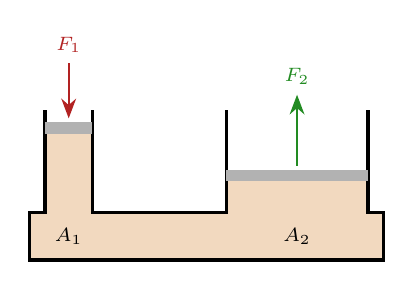
\begin{tikzpicture}[font=\scriptsize]
					\fill[cOrange!25] (0,0) rectangle (4.5,0.6);
					\fill[cOrange!25] (0.2,0.6) rectangle (0.8,1.6);
					\fill[cOrange!25] (2.5,0.6) rectangle (4.3,1.0);
					\draw[very thick] (0.2,1.9) -- (0.2,0.6) -- (0,0.6) -- (0,0) -- (4.5,0) -- (4.5,0.6) -- (4.3,0.6) -- (4.3,1.9);
					\draw[very thick] (0.8,1.9) -- (0.8,0.6) -- (2.5,0.6) -- (2.5,1.9);
					\fill[gray!60] (0.2,1.6) rectangle (0.8,1.75);
					\fill[gray!60] (2.5,1.0) rectangle (4.3,1.15);
					\draw[flowarrow, cRed] (0.5,2.5) -- (0.5,1.8) node[pos=0,above] {$F_1$};
					\draw[flowarrow, cGreen] (3.4,1.2) -- (3.4,2.1) node[above] {$F_2$};
					\node at (0.5,0.3) {$A_1$};
					\node at (3.4,0.3) {$A_2$};
				\end{tikzpicture}
			\end{column}
			\begin{column}{0.5\textwidth}
				\textbf{Example:} $F_1 = 100$ N on $A_1 = 10$ cm$^2$; $A_2 = 200$ cm$^2$.
				\[
				p = \frac{100}{10\times10^{-4}} = 10^5\ \text{Pa} = 1\ \text{bar}
				\]
				\[
				F_2 = 100\times\frac{200}{10} = \boxed{2000\ \text{N}}
				\]
				\footnotesize A 20$\times$ force gain --- but the big piston moves 20$\times$ \emph{less} distance (energy is conserved).
			\end{column}
		\end{columns}
	\end{frame}

	\begin{frame}{Elements of a Hydraulic System}
		\centering
		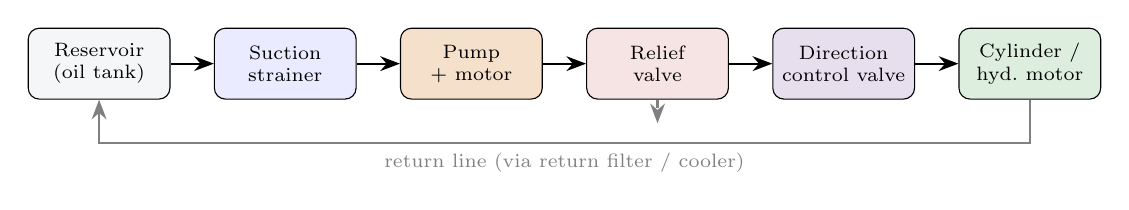
\begin{tikzpicture}[every node/.style={font=\scriptsize},
			el/.style={rectangle, draw=black, rounded corners, minimum width=1.8cm, minimum height=0.9cm, align=center, fill=blue!8}]
			\node[el, fill=cGrayBg] (tank) {Reservoir\\ (oil tank)};
			\node[el, right=0.55cm of tank] (filt) {Suction\\ strainer};
			\node[el, right=0.55cm of filt, fill=cOrange!20] (pump) {Pump\\ + motor};
			\node[el, right=0.55cm of pump, fill=cRed!12] (rv) {Relief\\ valve};
			\node[el, right=0.55cm of rv, fill=cPurple!15] (dcv) {Direction\\ control valve};
			\node[el, right=0.55cm of dcv, fill=cGreen!15] (act) {Cylinder /\\ hyd.\ motor};
			\draw[flowarrow] (tank) -- (filt);
			\draw[flowarrow] (filt) -- (pump);
			\draw[flowarrow] (pump) -- (rv);
			\draw[flowarrow] (rv) -- (dcv);
			\draw[flowarrow] (dcv) -- (act);
			\draw[flowarrow, gray] (act.south) -- ++(0,-0.55) -| node[pos=0.25, below] {return line (via return filter / cooler)} (tank.south);
			\draw[flowarrow, gray, dashed] (rv.south) -- ++(0,-0.3);
		\end{tikzpicture}
		\vspace{0.25cm}
		\begin{itemize}\small
			\item \textbf{Reservoir} --- stores oil, lets air escape and heat dissipate.
			\item \textbf{Pump} --- gear, vane or piston type; it creates \emph{flow}, the load creates \emph{pressure}.
			\item \textbf{Relief valve} --- the safety fuse: dumps oil to tank if pressure exceeds the setting.
			\item \textbf{Valves} direct and meter the oil; \textbf{actuators} convert it into force and motion.
			\item Unlike pneumatics, oil is \textbf{returned} to the tank --- it is a closed circuit.
		\end{itemize}
	\end{frame}

	\begin{frame}{Hydraulic Cylinder: Force and Speed}
		\begin{columns}[T]
			\begin{column}{0.5\textwidth}
				\begin{block}{Key formulas}
					\small
					\[
					F = p\,A, \qquad A = \frac{\pi D^2}{4}
					\]
					\[
					v = \frac{Q}{A} \qquad (Q = \text{flow rate})
					\]
					\[
					P_{\text{hyd}} = p\,Q \qquad (\text{power})
					\]
				\end{block}
				\footnotesize Force depends on \textbf{pressure}; speed depends on \textbf{flow}.
			\end{column}
			\begin{column}{0.5\textwidth}
				\textbf{Example:} bore $D = 100$ mm, $p = 100$ bar, $Q = 20$ L/min.
				\small
				\begin{align*}
					A &= \tfrac{\pi (0.1)^2}{4} = 7.854\times10^{-3}\ \text{m}^2\\
					F &= (100\times10^{5})(7.854\times10^{-3}) \approx \boxed{78.5\ \text{kN}}\\
					Q &= \tfrac{20\times10^{-3}}{60} = 3.33\times10^{-4}\ \text{m}^3/\text{s}\\
					v &= \tfrac{3.33\times10^{-4}}{7.854\times10^{-3}} \approx \boxed{42\ \text{mm/s}}\\
					P &= (10^7)(3.33\times10^{-4}) \approx 3.3\ \text{kW}
				\end{align*}
			\end{column}
		\end{columns}
	\end{frame}

	% =================================================================
	\section{Electrical Control Systems}
	% =================================================================
	\begin{frame}{Elements of an Electrical Control System}
		\centering
		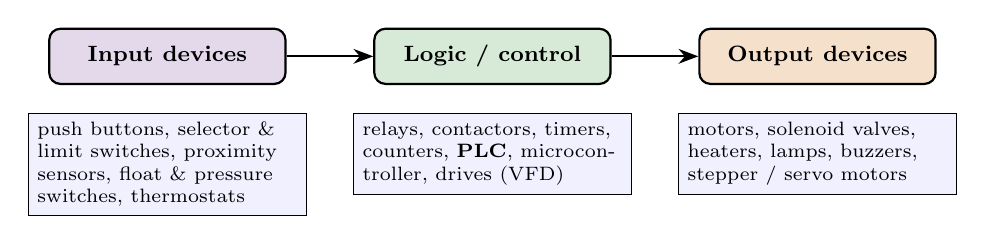
\begin{tikzpicture}[every node/.style={font=\footnotesize},
			hdr/.style={rectangle, draw=black, thick, rounded corners, minimum width=3.0cm, minimum height=0.7cm, align=center, font=\bfseries\footnotesize},
			grp/.style={rectangle, draw=black, align=left, fill=blue!6, text width=3.3cm, font=\scriptsize}]
			\node[hdr, fill=cPurple!18] (in) {Input devices};
			\node[hdr, right=1.1cm of in, fill=cGreen!18] (lo) {Logic / control};
			\node[hdr, right=1.1cm of lo, fill=cOrange!20] (out) {Output devices};
			\draw[flowarrow] (in) -- (lo);
			\draw[flowarrow] (lo) -- (out);
			\node[grp, below=0.35cm of in] {push buttons, selector \& limit switches, proximity sensors, float \& pressure switches, thermostats};
			\node[grp, below=0.35cm of lo] {relays, contactors, timers, counters, \textbf{PLC}, microcontroller, drives (VFD)};
			\node[grp, below=0.35cm of out] {motors, solenoid valves, heaters, lamps, buzzers, stepper / servo motors};
		\end{tikzpicture}
		\vspace{0.3cm}
		\begin{columns}[T]
			\begin{column}{0.5\textwidth}
				\begin{block}{Relay / contactor}
					\small An electrically operated switch: a small coil current (24 V) closes contacts that carry a large load current. A \textbf{contactor} is a heavy-duty relay for motors.
				\end{block}
			\end{column}
			\begin{column}{0.5\textwidth}
				\begin{block}{NO and NC contacts}
					\small \textbf{NO} (normally open) closes when operated; \textbf{NC} (normally closed) opens when operated. Stop buttons are always \textbf{NC} (fail-safe).
				\end{block}
			\end{column}
		\end{columns}
	\end{frame}

	\begin{frame}{The Programmable Logic Controller (PLC)}
		\begin{columns}[T]
			\begin{column}{0.55\textwidth}
				\begin{block}{PLC}
					A rugged industrial computer that reads \textbf{inputs}, runs a user \textbf{program} and sets \textbf{outputs}. It replaced large panels of hard-wired relays.
				\end{block}
				\begin{itemize}\small
					\item Programmed in IEC 61131-3 languages: \textbf{Ladder} (LD), Function Block (FBD), Structured Text (ST, looks like C/Pascal), \dots
					\item Changing the logic = editing software, not rewiring.
					\item Built-in timers, counters, PID blocks, communication.
				\end{itemize}
			\end{column}
			\begin{column}{0.45\textwidth}
				\centering
				\textbf{The PLC scan cycle}\\[4pt]
				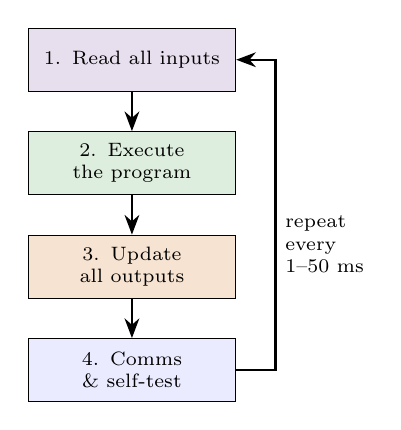
\begin{tikzpicture}[font=\scriptsize, node distance=0.5cm]
					\node[process, fill=cPurple!15, text width=2.4cm] (r) {1. Read all inputs};
					\node[process, fill=cGreen!15, below=of r, text width=2.4cm] (e) {2. Execute the program};
					\node[process, fill=cOrange!18, below=of e, text width=2.4cm] (w) {3. Update all outputs};
					\node[process, fill=blue!8, below=of w, text width=2.4cm] (h) {4. Comms \& self-test};
					\draw[flowarrow] (r) -- (e); \draw[flowarrow] (e) -- (w); \draw[flowarrow] (w) -- (h);
					\draw[flowarrow] (h.east) -- ++(0.5,0) |- (r.east);
					\node[right, align=left] at ($(h.east)+(0.5,1.6)$) {repeat\\ every\\ 1--50 ms};
				\end{tikzpicture}
			\end{column}
		\end{columns}
	\end{frame}

	\begin{frame}[fragile]{Ladder Logic: Motor Start/Stop (Seal-in) Circuit}
		\begin{columns}[T]
			\begin{column}{0.58\textwidth}
				\centering
				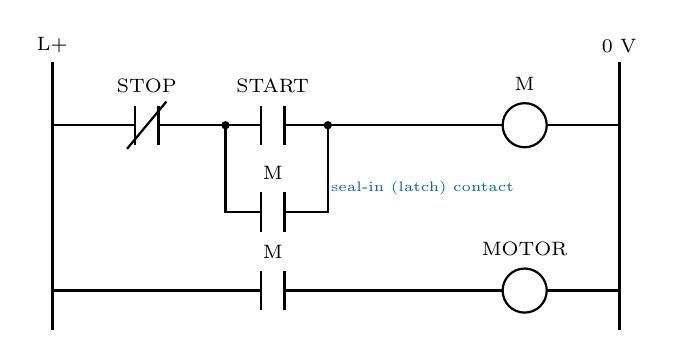
\begin{tikzpicture}[font=\scriptsize]
					% rails
					\draw[very thick] (0,0.8) -- (0,-2.6);
					\draw[very thick] (7.2,0.8) -- (7.2,-2.6);
					\node[above] at (0,0.8) {L+};
					\node[above] at (7.2,0.8) {0 V};
					% rung 1
					\draw[thick] (0,0) -- (1.05,0);
					\ladNC{1.2}{0}{STOP}
					\draw[thick] (1.35,0) -- (2.65,0);
					\ladNO{2.8}{0}{START}
					\draw[thick] (2.95,0) -- (5.72,0);
					\ladCoil{6.0}{0}{M}
					\draw[thick] (6.28,0) -- (7.2,0);
					% seal-in branch
					\draw[thick] (2.2,0) -- (2.2,-1.1) -- (2.65,-1.1);
					\ladNO{2.8}{-1.1}{M}
					\draw[thick] (2.95,-1.1) -- (3.5,-1.1) -- (3.5,0);
					\fill (2.2,0) circle (1.5pt);
					\fill (3.5,0) circle (1.5pt);
					% rung 2
					\draw[thick] (0,-2.1) -- (2.65,-2.1);
					\ladNO{2.8}{-2.1}{M}
					\draw[thick] (2.95,-2.1) -- (5.72,-2.1);
					\ladCoil{6.0}{-2.1}{MOTOR}
					\draw[thick] (6.28,-2.1) -- (7.2,-2.1);
					\node[font=\tiny, cAccent] at (4.7,-0.8) {seal-in (latch) contact};
				\end{tikzpicture}
			\end{column}
			\begin{column}{0.42\textwidth}
				\begin{itemize}\small
					\item Press \textbf{START} $\rightarrow$ coil \textbf{M} energises.
					\item Contact \textbf{M} in parallel keeps the coil ON after START is released --- the circuit \emph{remembers}.
					\item Press \textbf{STOP} (NC) $\rightarrow$ rung breaks, M drops out.
					\item Power failure also drops M --- motor won't restart by itself (safety).
				\end{itemize}
				\vspace{0.1cm}
				\textbf{Same logic as one C statement:}
\begin{lstlisting}
M = (START || M) && !STOP;
\end{lstlisting}
			\end{column}
		\end{columns}
	\end{frame}

	% =================================================================
	\section{Valves}
	% =================================================================
	\begin{frame}{Classification of Valves}
		\centering
		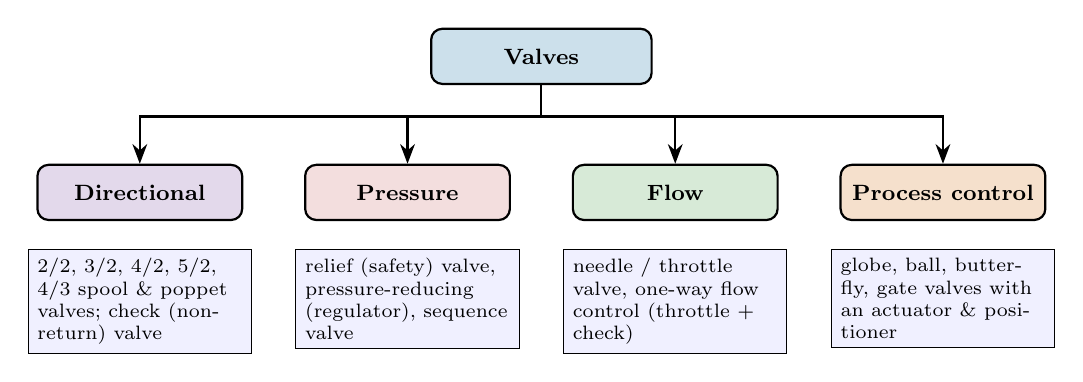
\begin{tikzpicture}[every node/.style={font=\footnotesize},
			hdr/.style={rectangle, draw=black, thick, rounded corners, minimum width=2.8cm, minimum height=0.7cm, align=center, font=\bfseries\footnotesize},
			grp/.style={rectangle, draw=black, align=left, fill=blue!6, text width=2.6cm, font=\scriptsize}]
			\node[hdr, fill=cAccent!20] (v) {Valves};
			\node[hdr, below=1.0cm of v, xshift=-5.1cm, fill=cPurple!18, minimum width=2.6cm] (d) {Directional};
			\node[hdr, below=1.0cm of v, xshift=-1.7cm, fill=cRed!15, minimum width=2.6cm] (p) {Pressure};
			\node[hdr, below=1.0cm of v, xshift=1.7cm, fill=cGreen!18, minimum width=2.6cm] (f) {Flow};
			\node[hdr, below=1.0cm of v, xshift=5.1cm, fill=cOrange!20, minimum width=2.6cm] (c) {Process control};
			\foreach \n in {d,p,f,c} \draw[flowarrow] (v.south) -- ++(0,-0.4) -| (\n.north);
			\node[grp, below=0.35cm of d] {2/2, 3/2, 4/2, 5/2, 4/3 spool \& poppet valves; check (non-return) valve};
			\node[grp, below=0.35cm of p] {relief (safety) valve, pressure-reducing (regulator), sequence valve};
			\node[grp, below=0.35cm of f] {needle / throttle valve, one-way flow control (throttle + check)};
			\node[grp, below=0.35cm of c] {globe, ball, butterfly, gate valves with an actuator \& positioner};
		\end{tikzpicture}
		\vspace{0.3cm}
		\begin{itemize}\small
			\item \textbf{Directional} valves decide \emph{where} fluid goes (ON/OFF --- logic control).
			\item \textbf{Pressure} and \textbf{flow} valves decide \emph{how hard} and \emph{how fast}.
			\item \textbf{Process control} valves throttle continuously --- they are the final control element of a PID loop.
		\end{itemize}
	\end{frame}

	\begin{frame}{Directional Control Valves: Ports / Positions}
		\begin{block}{Naming rule}
			A valve is named \textbf{``ports / positions''}: a \textbf{3/2 valve} has 3 ports and 2 switching positions.
			Port numbers (ISO 5599): \textbf{1} = supply, \textbf{2, 4} = outputs, \textbf{3, 5} = exhausts.
		\end{block}
		\vspace{0.1cm}
		\centering
		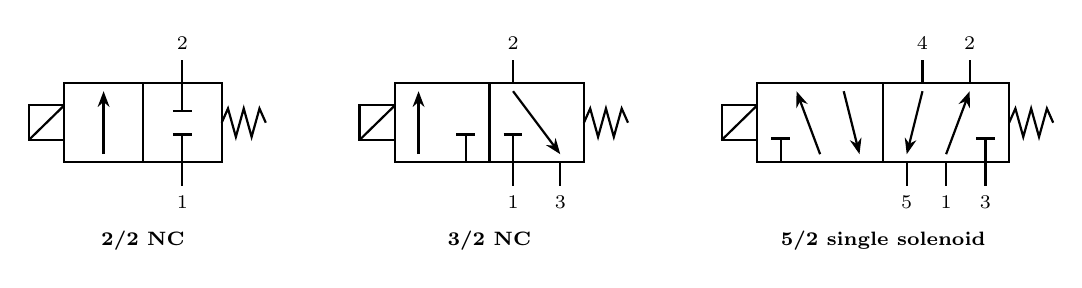
\begin{tikzpicture}[font=\scriptsize]
			% ---------------- 2/2 NC ----------------
			\begin{scope}[shift={(0,0)}]
				\draw[thick] (0,0) rectangle (1.0,1.0);
				\draw[thick] (1.0,0) rectangle (2.0,1.0);
				\draw[vflow] (0.5,0.1) -- (0.5,0.9);
				\vblock{1.5}{0}{0.35}
				\vblock{1.5}{1}{-0.35}
				\draw[thick] (1.5,0) -- (1.5,-0.3) node[below] {1};
				\draw[thick] (1.5,1) -- (1.5,1.3) node[above] {2};
				\vsolenoid{0}{0.5}
				\vspring{2.0}{0.5}
				\node at (1.0,-1.0) {\textbf{2/2 NC}};
			\end{scope}
			% ---------------- 3/2 NC ----------------
			\begin{scope}[shift={(4.2,0)}]
				\draw[thick] (0,0) rectangle (1.2,1.0);
				\draw[thick] (1.2,0) rectangle (2.4,1.0);
				\draw[vflow] (0.3,0.1) -- (0.3,0.9);
				\vblock{0.9}{0}{0.35}
				\draw[vflow] (1.5,0.9) -- (2.1,0.1);
				\vblock{1.5}{0}{0.35}
				\draw[thick] (1.5,0) -- (1.5,-0.3) node[below] {1};
				\draw[thick] (2.1,0) -- (2.1,-0.3) node[below] {3};
				\draw[thick] (1.5,1) -- (1.5,1.3) node[above] {2};
				\vsolenoid{0}{0.5}
				\vspring{2.4}{0.5}
				\node at (1.2,-1.0) {\textbf{3/2 NC}};
			\end{scope}
			% ---------------- 5/2 ----------------
			\begin{scope}[shift={(8.8,0)}]
				\draw[thick] (0,0) rectangle (1.6,1.0);
				\draw[thick] (1.6,0) rectangle (3.2,1.0);
				\draw[vflow] (0.8,0.1) -- (0.5,0.9);
				\draw[vflow] (1.1,0.9) -- (1.3,0.1);
				\vblock{0.3}{0}{0.3}
				\draw[vflow] (2.4,0.1) -- (2.7,0.9);
				\draw[vflow] (2.1,0.9) -- (1.9,0.1);
				\vblock{2.9}{0}{0.3}
				\draw[thick] (1.9,0) -- (1.9,-0.3) node[below] {5};
				\draw[thick] (2.4,0) -- (2.4,-0.3) node[below] {1};
				\draw[thick] (2.9,0) -- (2.9,-0.3) node[below] {3};
				\draw[thick] (2.1,1) -- (2.1,1.3) node[above] {4};
				\draw[thick] (2.7,1) -- (2.7,1.3) node[above] {2};
				\vsolenoid{0}{0.5}
				\vspring{3.2}{0.5}
				\node at (1.6,-1.0) {\textbf{5/2 single solenoid}};
			\end{scope}
		\end{tikzpicture}
		\vspace{0.1cm}
		\begin{itemize}\small
			\item \textbf{2/2} --- simple ON/OFF tap. \quad \textbf{3/2} --- drives a \emph{single-acting} cylinder. \quad \textbf{5/2} --- drives a \emph{double-acting} cylinder.
			\item Actuation: manual (button, lever), mechanical (roller), \textbf{solenoid}, pilot air; return usually by \textbf{spring}.
		\end{itemize}
	\end{frame}

	\begin{frame}{Process Control Valves}
		\begin{columns}[T]
			\begin{column}{0.45\textwidth}
				\centering
				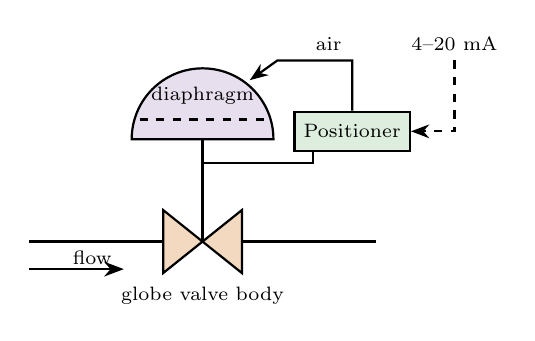
\begin{tikzpicture}[font=\scriptsize]
					% pipe and globe valve body
					\draw[very thick] (-2.2,0) -- (-0.5,0);
					\draw[very thick] (0.5,0) -- (2.2,0);
					\filldraw[fill=cOrange!25, thick] (-0.5,-0.4) -- (-0.5,0.4) -- (0.5,-0.4) -- (0.5,0.4) -- cycle;
					% stem
					\draw[very thick] (0,0) -- (0,1.3);
					% diaphragm actuator
					\filldraw[fill=cPurple!15, thick] (-0.9,1.3) -- (0.9,1.3) arc (0:180:0.9) -- cycle;
					\draw[thick, dashed] (-0.8,1.55) -- (0.8,1.55);
					\node at (0,1.85) {diaphragm};
					% positioner
					\node[rectangle, draw, thick, fill=cGreen!15, minimum width=1cm, minimum height=0.5cm] (pos) at (1.9,1.4) {Positioner};
					\draw[thick] (0,1.0) -- (1.4,1.0) -- (1.4,1.15);
					\draw[dashed, thick, -{Stealth}] (3.2,2.3) node[above] {4--20 mA} |- (pos.east);
					\draw[thick, -{Stealth}] (pos.north) |- (0.95,2.3) -- (0.6,2.05);
					\node[above] at (1.6,2.3) {air};
					\node[below] at (-1.4,0) {flow};
					\draw[flowarrow] (-2.2,-0.35) -- (-1.0,-0.35);
					\node[below] at (0,-0.45) {globe valve body};
				\end{tikzpicture}
			\end{column}
			\begin{column}{0.55\textwidth}
				\begin{itemize}\small
					\item \textbf{Body}: globe (fine throttling), ball, butterfly (large pipes), gate (isolation only).
					\item \textbf{Actuator}: diaphragm (air), piston, or electric motor moves the stem.
					\item \textbf{Positioner}: converts the 4--20 mA controller signal into accurate stem position.
				\end{itemize}
				\begin{block}{Fail-safe action}
					\small \textbf{Air-to-open} (fail-closed) --- e.g.\ fuel valve closes if air is lost.\\
					\textbf{Air-to-close} (fail-open) --- e.g.\ cooling-water valve opens if air is lost.
				\end{block}
			\end{column}
		\end{columns}
	\end{frame}

	\begin{frame}{Control Valve Characteristics and Sizing}
		\begin{columns}[T]
			\begin{column}{0.48\textwidth}
				\centering
				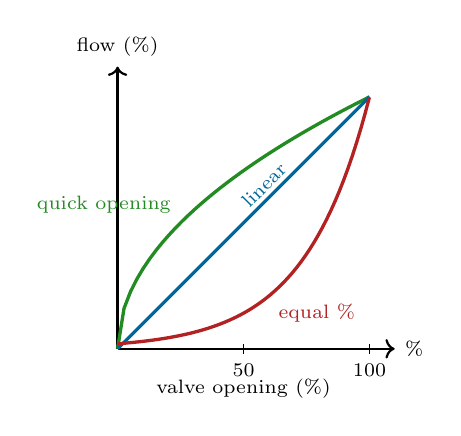
\begin{tikzpicture}[font=\scriptsize, scale=3.2]
					\draw[->, thick] (0,0) -- (1.1,0) node[right] {\%};
					\node[below] at (0.5,-0.08) {valve opening (\%)};
					\draw[->, thick] (0,0) -- (0,1.12) node[above] {flow (\%)};
					\draw[very thick, cGreen, domain=0:1, samples=40] plot (\x, {sqrt(\x)});
					\draw[very thick, cAccent] (0,0) -- (1,1);
					\draw[very thick, cRed, domain=0:1, samples=60] plot (\x, {50^(\x-1)});
					\node[cGreen, above left] at (0.25,0.5) {quick opening};
					\node[cAccent, rotate=45] at (0.58,0.65) {linear};
					\node[cRed, right] at (0.6,0.14) {equal \%};
					\foreach \t in {0.5,1} {\draw (\t,0.02) -- (\t,-0.02) node[below] {\pgfmathparse{int(\t*100)}\pgfmathresult};}
				\end{tikzpicture}
			\end{column}
			\begin{column}{0.52\textwidth}
				\begin{itemize}\small
					\item \textbf{Linear}: flow $\propto$ opening --- level loops.
					\item \textbf{Equal percentage}: each step adds the same \emph{\%} of current flow --- most common for pressure / flow loops.
					\item \textbf{Quick opening}: nearly full flow at small opening --- ON/OFF service.
				\end{itemize}
				\begin{block}{Sizing: flow coefficient $C_v$}
					\small
					\[
					Q = C_v\sqrt{\frac{\Delta p}{SG}}\quad(\text{US gpm, psi})
					\]
					$C_v = 10$, $\Delta p = 16$ psi, water ($SG=1$): $Q = 10\sqrt{16} = \boxed{40\ \text{gpm}}$
				\end{block}
			\end{column}
		\end{columns}
	\end{frame}

	% =================================================================
	\section{Actuators}
	% =================================================================
	\begin{frame}{Classification of Actuators}
		\begin{block}{Actuator}
			A device that converts an energy source (air, oil, electricity) into \textbf{mechanical motion} --- the ``muscles'' of an automated system.
		\end{block}
		\centering
		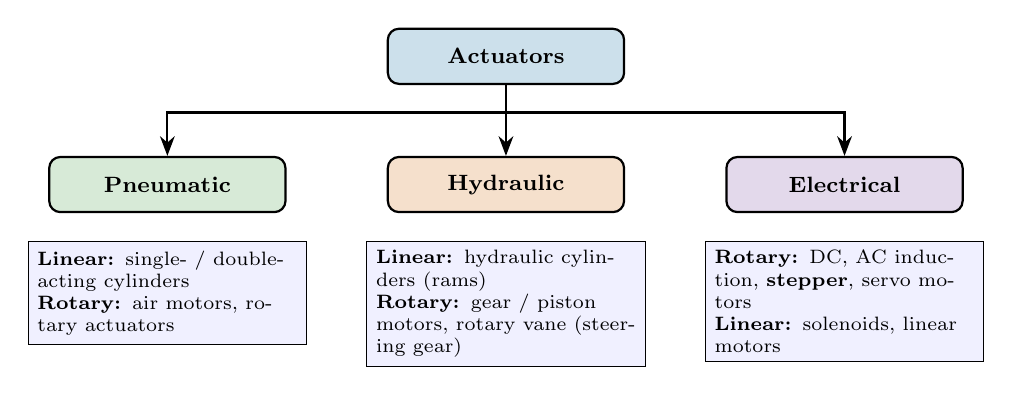
\begin{tikzpicture}[every node/.style={font=\footnotesize},
			hdr/.style={rectangle, draw=black, thick, rounded corners, minimum width=3.0cm, minimum height=0.7cm, align=center, font=\bfseries\footnotesize},
			grp/.style={rectangle, draw=black, align=left, fill=blue!6, text width=3.3cm, font=\scriptsize}]
			\node[hdr, fill=cAccent!20] (a) {Actuators};
			\node[hdr, below=0.9cm of a, xshift=-4.3cm, fill=cGreen!18] (pn) {Pneumatic};
			\node[hdr, below=0.9cm of a, fill=cOrange!20] (hy) {Hydraulic};
			\node[hdr, below=0.9cm of a, xshift=4.3cm, fill=cPurple!18] (el) {Electrical};
			\foreach \n in {pn,hy,el} \draw[flowarrow] (a.south) -- ++(0,-0.35) -| (\n.north);
			\node[grp, below=0.35cm of pn] {\textbf{Linear:} single- / double-acting cylinders\\ \textbf{Rotary:} air motors, rotary actuators};
			\node[grp, below=0.35cm of hy] {\textbf{Linear:} hydraulic cylinders (rams)\\ \textbf{Rotary:} gear / piston motors, rotary vane (steering gear)};
			\node[grp, below=0.35cm of el] {\textbf{Rotary:} DC, AC induction, \textbf{stepper}, servo motors\\ \textbf{Linear:} solenoids, linear motors};
		\end{tikzpicture}
	\end{frame}

	\begin{frame}{Linear Actuators: Cylinders}
		\begin{columns}[T]
			\begin{column}{0.5\textwidth}
				\centering
				\textbf{Single-acting} (spring return)\\[4pt]
				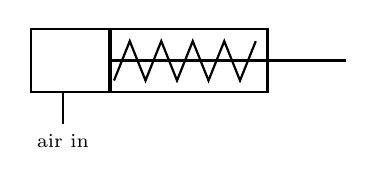
\begin{tikzpicture}[font=\scriptsize]
					\draw[thick] (0,0) rectangle (3,0.8);
					\draw[very thick] (1.0,0) -- (1.0,0.8);
					\draw[very thick] (1.0,0.4) -- (4.0,0.4);
					\draw[thick] (1.05,0.15) -- ++(0.2,0.5) -- ++(0.2,-0.5) -- ++(0.2,0.5) -- ++(0.2,-0.5) -- ++(0.2,0.5) -- ++(0.2,-0.5) -- ++(0.2,0.5) -- ++(0.2,-0.5) -- ++(0.2,0.5);
					\draw[thick] (0.4,0) -- (0.4,-0.4) node[below] {air in};
				\end{tikzpicture}
				\vspace{0.2cm}

				\textbf{Double-acting}\\[4pt]
				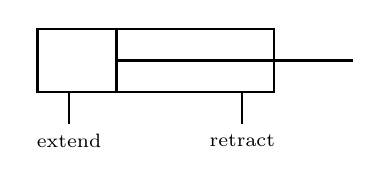
\begin{tikzpicture}[font=\scriptsize]
					\draw[thick] (0,0) rectangle (3,0.8);
					\draw[very thick] (1.0,0) -- (1.0,0.8);
					\draw[very thick] (1.0,0.4) -- (4.0,0.4);
					\draw[thick] (0.4,0) -- (0.4,-0.4) node[below] {extend};
					\draw[thick] (2.6,0) -- (2.6,-0.4) node[below] {retract};
				\end{tikzpicture}
			\end{column}
			\begin{column}{0.5\textwidth}
				\textbf{Example:} pneumatic cylinder, bore $D = 50$ mm, rod $d = 20$ mm, $p = 6$ bar (0.6 N/mm$^2$).
				\small
				\begin{align*}
					A_{\text{cap}} &= \tfrac{\pi}{4}(50)^2 = 1963\ \text{mm}^2\\
					F_{\text{ext}} &= 0.6\times1963 \approx \boxed{1178\ \text{N}}\\
					A_{\text{ann}} &= \tfrac{\pi}{4}(50^2 - 20^2) = 1649\ \text{mm}^2\\
					F_{\text{ret}} &= 0.6\times1649 \approx \boxed{990\ \text{N}}
				\end{align*}
				\footnotesize Retracting force is \textbf{smaller} because the rod takes up part of the piston area. (Real force $\approx$ 10\,\% less due to friction.)
			\end{column}
		\end{columns}
	\end{frame}

	\begin{frame}{Electrical Actuators at a Glance}
		\renewcommand{\arraystretch}{1.35}
		\centering
		\small
		\begin{tabular}{@{}p{2.6cm}p{4.2cm}p{2.6cm}p{3.6cm}@{}}
			\toprule
			\textbf{Actuator} & \textbf{Principle} & \textbf{Control} & \textbf{Typical use} \\
			\midrule
			Solenoid          & coil pulls an iron plunger       & ON/OFF        & valve pilots, door locks \\
			DC motor          & current in a magnetic field      & voltage / PWM & fans, small drives, toys \\
			AC induction motor& rotating magnetic field          & VFD (frequency) & pumps, compressors, winches \\
			\textbf{Stepper motor} & moves in fixed angular steps & pulses (open loop) & 3D printers, valves, CNC \\
			Servo motor       & motor + encoder feedback         & closed loop (PID) & robots, CNC axes \\
			\bottomrule
		\end{tabular}
		\vspace{0.4cm}
		\begin{block}{Key idea}
			When \textbf{position} must be controlled precisely, we use either a \textbf{stepper} (count the pulses, no feedback needed) or a \textbf{servo} (measure the position and correct it with PID).
		\end{block}
	\end{frame}

	% =================================================================
	\section{Stepper Motors}
	% =================================================================
	\begin{frame}{What is a Stepper Motor?}
		\begin{columns}[T]
			\begin{column}{0.55\textwidth}
				\begin{block}{Stepper motor}
					A brushless motor that rotates in \textbf{discrete, equal angular steps}. Each input \textbf{pulse} moves the shaft by one \textbf{step angle}.
				\end{block}
				\begin{itemize}\small
					\item Position $=$ number of pulses $\times$ step angle.
					\item Speed $\propto$ pulse frequency.
					\item Direction set by the \emph{order} in which coils are energised.
					\item Runs \textbf{open loop} --- no position sensor needed (if not overloaded).
					\item Holds position firmly when stopped (\textbf{holding torque}).
				\end{itemize}
			\end{column}
			\begin{column}{0.45\textwidth}
				\centering
				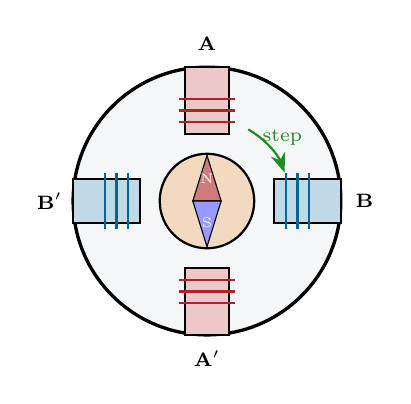
\begin{tikzpicture}[font=\scriptsize]
					\draw[very thick, fill=cGrayBg] (0,0) circle (1.7);
					\foreach \ang/\lab/\col in {90/A/cRed, 0/B/cAccent, 270/{A$'$}/cRed, 180/{B$'$}/cAccent} {
						\begin{scope}[rotate=\ang]
							\filldraw[fill=\col!25, thick] (0.85,-0.28) rectangle (1.7,0.28);
							\draw[\col, thick] (1.0,-0.36) -- (1.0,0.36) (1.15,-0.36) -- (1.15,0.36) (1.3,-0.36) -- (1.3,0.36);
						\end{scope}
						\node at (\ang:2.0) {\textbf{\lab}};
					}
					\filldraw[fill=cOrange!25, thick] (0,0) circle (0.6);
					\filldraw[fill=cRed!60] (0,0) -- (-0.18,0) -- (0,0.58) -- (0.18,0) -- cycle;
					\filldraw[fill=blue!40] (0,0) -- (-0.18,0) -- (0,-0.58) -- (0.18,0) -- cycle;
					\node[white] at (0,0.28) {\tiny N};
					\node[white] at (0,-0.28) {\tiny S};
					\draw[flowarrow, cGreen] (60:1.05) arc (60:20:1.05);
					\node[cGreen] at (40:1.25) {step};
				\end{tikzpicture}

				\footnotesize Coil A energised $\rightarrow$ rotor aligns with A.\\ Next pulse energises B $\rightarrow$ rotor turns 90$^\circ$.
			\end{column}
		\end{columns}
	\end{frame}

	\begin{frame}{Types of Stepper Motors}
		\begin{columns}[T]
			\begin{column}{0.32\textwidth}
				\begin{block}{Permanent Magnet (PM)}
					\begin{itemize}\small
						\item Rotor is a permanent magnet.
						\item Step angle 7.5$^\circ$--15$^\circ$.
						\item Low cost, low speed; has detent torque.
						\item Printers, small valves.
					\end{itemize}
				\end{block}
			\end{column}
			\begin{column}{0.32\textwidth}
				\begin{block}{Variable Reluctance (VR)}
					\begin{itemize}\small
						\item Toothed soft-iron rotor, no magnet.
						\item Rotor moves to the position of \textbf{least reluctance}.
						\item No detent torque.
						\item $\theta = \dfrac{N_s - N_r}{N_s N_r}\times360^\circ$
					\end{itemize}
				\end{block}
			\end{column}
			\begin{column}{0.32\textwidth}
				\begin{block}{Hybrid}
					\begin{itemize}\small
						\item Magnet + toothed rotor.
						\item Fine steps: 1.8$^\circ$ (200 steps/rev) or 0.9$^\circ$.
						\item High torque \& accuracy.
						\item CNC, 3D printers, robots.
					\end{itemize}
				\end{block}
			\end{column}
		\end{columns}
		\vspace{0.3cm}
		\begin{block}{Example (VR motor)}
			\small Stator teeth $N_s = 8$, rotor teeth $N_r = 6$:\quad
			$\theta = \dfrac{8-6}{8\times6}\times360^\circ = \boxed{15^\circ}$ \quad $\Rightarrow$ \quad $360/15 = 24$ steps per revolution.
		\end{block}
	\end{frame}

	\begin{frame}{Drive Modes and Switching Sequence}
		\begin{columns}[T]
			\begin{column}{0.5\textwidth}
				\renewcommand{\arraystretch}{1.2}
				\centering
				\small
				\begin{tabular}{@{}lll@{}}
					\toprule
					\textbf{Mode} & \textbf{Coils ON} & \textbf{Step} \\
					\midrule
					Wave drive  & one at a time          & full, low torque \\
					Full step   & two at a time          & full, max torque \\
					Half step   & one \& two alternately & half ($0.9^\circ$) \\
					Micro-step  & sine/cosine currents   & $1/16$, $1/256$ \dots \\
					\bottomrule
				\end{tabular}
				\vspace{0.3cm}

				\renewcommand{\arraystretch}{1.1}
				\begin{tabular}{@{}c|cccc|c@{}}
					\multicolumn{6}{c}{\textbf{Full-step (two-phase ON) sequence}}\\
					\toprule
					Step & A & B & A$'$ & B$'$ & Rotor \\
					\midrule
					1 & 1 & 1 & 0 & 0 & 45$^\circ$ \\
					2 & 0 & 1 & 1 & 0 & 135$^\circ$ \\
					3 & 0 & 0 & 1 & 1 & 225$^\circ$ \\
					4 & 1 & 0 & 0 & 1 & 315$^\circ$ \\
					\bottomrule
				\end{tabular}
			\end{column}
			\begin{column}{0.5\textwidth}
				\centering
				\textbf{Wave-drive pulse timing}\\[6pt]
				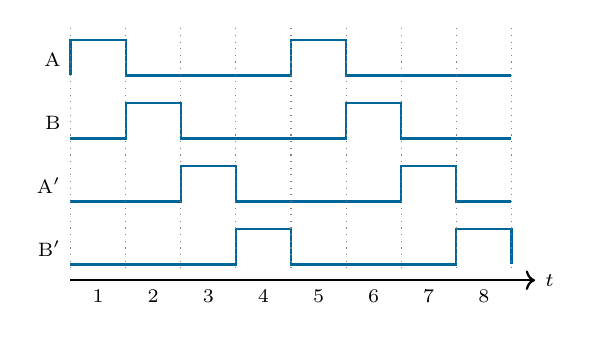
\begin{tikzpicture}[font=\scriptsize]
					\foreach \name/\row/\off in {A/0/0, B/1/1, {A$'$}/2/2, {B$'$}/3/3} {
						\pgfmathsetmacro{\y}{-\row*0.8}
						\node[left] at (0,\y+0.2) {\name};
						\draw[thick, cAccent] (0,\y) -- ++(\off*0.7,0) -- ++(0,0.45) -- ++(0.7,0) -- ++(0,-0.45)
						-- ++(2.1,0) -- ++(0,0.45) -- ++(0.7,0) -- ++(0,-0.45) -- ++({(3-\off)*0.7},0);
					}
					\foreach \k in {0,...,8} \draw[gray, dotted] (\k*0.7,0.6) -- (\k*0.7,-2.5);
					\draw[->, thick] (0,-2.6) -- (5.9,-2.6) node[right] {$t$};
					\foreach \k in {1,...,8} \node[below] at ({(\k-0.5)*0.7},-2.6) {\k};
				\end{tikzpicture}

				\vspace{0.2cm}
				\footnotesize Reversing the order (B$'$, A$'$, B, A) reverses the direction.
			\end{column}
		\end{columns}
	\end{frame}

	\begin{frame}{Stepper Motor Calculations}
		\begin{block}{Useful relations}
			\[
			\text{Steps/rev} = \frac{360^\circ}{\theta}
			\qquad
			\text{Speed (rpm)} = \frac{f\,\theta}{6}
			\qquad
			\text{Linear step} = \frac{\text{lead-screw pitch}}{\text{steps/rev}}
			\]
			$\theta$ = step angle (degrees), $f$ = pulse rate (pulses/s).
		\end{block}
		\begin{columns}[T]
			\begin{column}{0.5\textwidth}
				\textbf{Example:} hybrid motor, $\theta = 1.8^\circ$, driven at $f = 1000$ pulses/s.
				\small
				\begin{align*}
					\text{Steps/rev} &= 360/1.8 = 200\\
					\text{rev/s} &= 1000/200 = 5\\
					\text{Speed} &= \tfrac{1000\times1.8}{6} = \boxed{300\ \text{rpm}}
				\end{align*}
			\end{column}
			\begin{column}{0.5\textwidth}
				\textbf{Example:} same motor drives a lead screw of pitch 5 mm.
				\small
				\begin{align*}
					\text{Resolution} &= 5/200 = \boxed{0.025\ \text{mm/step}}\\
					\text{Pulses for 30 mm} &= 30/0.025 = 1200
				\end{align*}
				\footnotesize With 1/16 micro-stepping the resolution becomes 0.0016 mm.
			\end{column}
		\end{columns}
	\end{frame}

	\begin{frame}[fragile]{Driving a Stepper Motor}
		\begin{columns}[T]
			\begin{column}{0.46\textwidth}
				\centering
				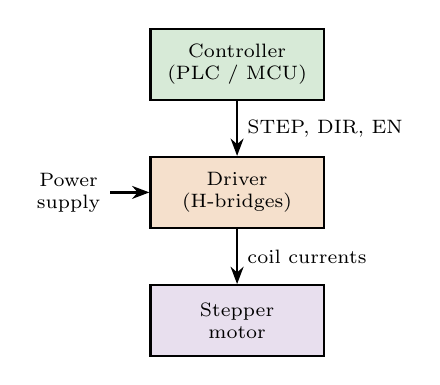
\begin{tikzpicture}[font=\scriptsize, node distance=0.7cm]
					\node[blk, fill=cGreen!18, minimum width=2.2cm] (mcu) {Controller\\ (PLC / MCU)};
					\node[blk, below=of mcu, fill=cOrange!20, minimum width=2.2cm] (drv) {Driver\\ (H-bridges)};
					\node[blk, below=of drv, fill=cPurple!15, minimum width=2.2cm] (mot) {Stepper\\ motor};
					\node[left=0.5cm of drv, align=center] (ps) {Power\\ supply};
					\draw[sig] (mcu) -- node[right] {STEP, DIR, EN} (drv);
					\draw[sig] (drv) -- node[right] {coil currents} (mot);
					\draw[sig] (ps) -- (drv);
				\end{tikzpicture}
				\vspace{0.2cm}

				\footnotesize The controller only sends \textbf{STEP} pulses and a \textbf{DIR} level; the driver switches the coil currents.
			\end{column}
			\begin{column}{0.54\textwidth}
				\begin{block}{Advantages}
					\small Precise open-loop positioning, excellent holding torque, simple digital control, long life (no brushes).
				\end{block}
				\begin{block}{Limitations}
					\small Torque falls at high speed; \textbf{missed steps} if overloaded (controller does not know!); resonance \& vibration; draws current even at standstill.
				\end{block}
				\footnotesize Critical positioning (e.g.\ a ship's fuel rack) adds an encoder to detect lost steps.
			\end{column}
		\end{columns}
	\end{frame}

	\begin{frame}[fragile, plain]{}

		\vspace*{0.05cm}

		\begin{columns}[T,onlytextwidth]

			% =========================================================
			% LEFT COLUMN -- PSEUDOCODE
			% =========================================================

			\begin{column}{0.28\textwidth}

				\begin{block}{Pseudocode}
					\scriptsize
					\begin{enumerate}
						\item START
						\item Set step angle \texttt{= 1.8}
						\item READ target \texttt{angle}
						\item \texttt{n = angle / 1.8} (rounded)
						\item PRINT \texttt{n}
						\item \textbf{FOR} \texttt{i = 1} to \texttt{n}
						\begin{itemize}\scriptsize
							\item Output pattern \texttt{seq[i mod 4]} to coils A, B, A$'$, B$'$
						\end{itemize}
						\item STOP
					\end{enumerate}
				\end{block}

			\end{column}


			% =========================================================
			% MIDDLE COLUMN -- C PROGRAM
			% =========================================================
			\hspace*{0.3cm}
			\begin{column}{0.44\textwidth}

				\begin{block}{C Program (wave-drive sequence)}

\begin{lstlisting}[style=cstyle,numbers=none,basicstyle=\ttfamily\scriptsize]
#include <stdio.h>

int main(void)
{
	float step = 1.8, angle;
	int   n, i;
	/* coil pattern: A B A' B' */
	const char *seq[4] =
		{"1000", "0100", "0010", "0001"};

	printf("Enter angle (deg): ");
	scanf("%f", &angle);

	n = (int)(angle / step + 0.5);
	printf("Steps needed = %d\n", n);

	for (i = 0; i < 8 && i < n; i++)
		printf("Step %d : %s\n", i+1, seq[i%4]);
	return 0;
}
\end{lstlisting}

				\end{block}

			\end{column}


			% =========================================================
			% RIGHT COLUMN -- OUTPUT
			% =========================================================

			\begin{column}{0.24\textwidth}

				\begin{tikzpicture}[remember picture,overlay]

					\node[
					anchor=north east,
					draw,
					rounded corners=2pt,
					fill=white,
					text width=3.4cm,
					align=left,
					inner sep=6pt
					] at ([xshift=-2mm,yshift=-6mm]current page.north east)
					{
						\textbf{Program Output}\\[3pt]
						\ttfamily\scriptsize
						Enter angle (deg): 90\\
						Steps needed = 50\\
						Step 1 : 1000\\
						Step 2 : 0100\\
						Step 3 : 0010\\
						Step 4 : 0001\\
						Step 5 : 1000\\
						Step 6 : 0100\\
						Step 7 : 0010\\
						Step 8 : 0001
					};

				\end{tikzpicture}

			\end{column}

		\end{columns}

		\begin{tikzpicture}[remember picture,overlay]
			\node[
			anchor=south east,
			draw,
			rounded corners=2pt,
			fill=cGrayBg,
			text width=3.4cm,
			align=left,
			inner sep=6pt,
			font=\scriptsize
			] at ([xshift=-2mm,yshift=4mm]current page.south east)
			{
				\textbf{Note:} only the first 8 of the 50 patterns are printed. On a real controller each \texttt{printf} is replaced by writing the 4 bits to an output port, followed by a short delay that sets the speed.
			};
		\end{tikzpicture}

	\end{frame}

	% =================================================================
	\section{PID Controllers}
	% =================================================================
	\begin{frame}{The Simplest Controller: ON--OFF}
		\begin{columns}[T]
			\begin{column}{0.48\textwidth}
				\begin{block}{ON--OFF (two-position) control}
					\small Output is either \textbf{100\,\%} or \textbf{0\,\%}. A \textbf{dead band} (hysteresis) prevents rapid chattering.
				\end{block}
				\begin{itemize}\small
					\item Example: fridge, water heater, bilge pump with float switch.
					\item Cheap and simple.
					\item But PV \textbf{always oscillates} around the setpoint, and the actuator wears out.
				\end{itemize}
				\vspace{0.1cm}
				\footnotesize For smooth, accurate control we need an output that varies \emph{continuously} with the error $\rightarrow$ \textbf{PID}.
			\end{column}
			\begin{column}{0.52\textwidth}
				\centering
				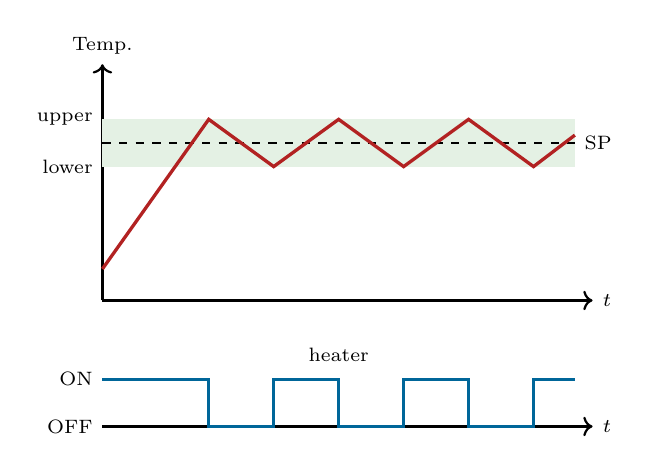
\begin{tikzpicture}[font=\scriptsize, x=0.75cm, y=1cm]
					% temperature
					\draw[->, thick] (0,0) -- (8.3,0) node[right] {$t$};
					\draw[->, thick] (0,0) -- (0,3.0) node[above] {Temp.};
					\fill[cGreen!12] (0,1.7) rectangle (8,2.3);
					\draw[dashed] (0,2.0) -- (8,2.0) node[right] {SP};
					\node[left] at (0,2.3) {upper};
					\node[left] at (0,1.7) {lower};
					\draw[very thick, cRed] (0,0.4) -- (1.8,2.3) -- (2.9,1.7) -- (4.0,2.3) -- (5.1,1.7) -- (6.2,2.3) -- (7.3,1.7) -- (8,2.1);
					% heater state
					\draw[->, thick] (0,-1.6) -- (8.3,-1.6) node[right] {$t$};
					\node[left] at (0,-1.0) {ON};
					\node[left] at (0,-1.6) {OFF};
					\draw[very thick, cAccent] (0,-1.0) -- (1.8,-1.0) -- (1.8,-1.6) -- (2.9,-1.6) -- (2.9,-1.0) -- (4.0,-1.0) -- (4.0,-1.6) -- (5.1,-1.6) -- (5.1,-1.0) -- (6.2,-1.0) -- (6.2,-1.6) -- (7.3,-1.6) -- (7.3,-1.0) -- (8,-1.0);
					\node[above] at (4.0,-0.9) {heater};
				\end{tikzpicture}
			\end{column}
		\end{columns}
	\end{frame}

	\begin{frame}{The PID Controller}
		\vspace*{-0.2cm}
		\begin{block}{PID control law}
			\[
			u(t) = \underbrace{K_p\,e(t)}_{\text{Proportional}} + \underbrace{K_i\!\int_0^t e(\tau)\,d\tau}_{\text{Integral}} + \underbrace{K_d\,\frac{de(t)}{dt}}_{\text{Derivative}},
			\qquad e(t) = \text{SP} - \text{PV}
			\]
		\end{block}
		\centering
		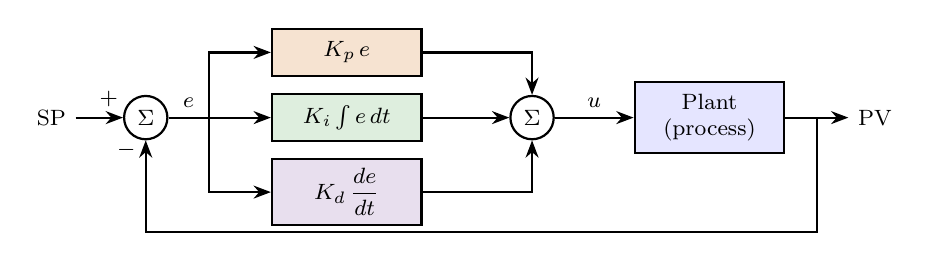
\begin{tikzpicture}[font=\footnotesize, node distance=0.9cm]
			\node (r) {SP};
			\node[sumj, right=0.6cm of r] (s1) {$\Sigma$};
			\node[blk, right=1.3cm of s1, fill=cGreen!15, minimum height=0.6cm] (i) {$K_i\int e\,dt$};
			\node[blk, above=0.2cm of i, fill=cOrange!18, minimum height=0.6cm] (p) {$K_p\,e$};
			\node[blk, below=0.2cm of i, fill=cPurple!15, minimum height=0.6cm] (d) {$K_d\,\dfrac{de}{dt}$};
			\node[sumj, right=1.1cm of i] (s2) {$\Sigma$};
			\node[blk, right=1.0cm of s2, fill=blue!10] (pl) {Plant\\ (process)};
			\node[right=0.8cm of pl] (y) {PV};
			\draw[sig] (r) -- node[above, pos=0.7] {$+$} (s1);
			\draw[thick] (s1) -- node[above] {$e$} ++(0.8,0) coordinate (br);
			\draw[sig] (br) |- (p.west);
			\draw[sig] (br) -- (i.west);
			\draw[sig] (br) |- (d.west);
			\draw[sig] (p.east) -| (s2.north);
			\draw[sig] (i.east) -- (s2.west);
			\draw[sig] (d.east) -| (s2.south);
			\draw[sig] (s2) -- node[above] {$u$} (pl);
			\draw[sig] (pl) -- coordinate[pos=0.5] (tap) (y);
			\draw[sig] (tap) -- ++(0,-1.45) -| node[left, pos=0.95] {$-$} (s1.south);
		\end{tikzpicture}
		\vspace{0.15cm}

		\small Industrial (standard) form: \quad $u = K_p\left(e + \dfrac{1}{T_i}\displaystyle\int e\,dt + T_d\dfrac{de}{dt}\right)$, \quad $K_i = \dfrac{K_p}{T_i}$, \; $K_d = K_p T_d$
	\end{frame}

	\begin{frame}{P, I and D Actions: What Each Term Does}
		\begin{columns}[T]
			\begin{column}{0.32\textwidth}
				\begin{block}{P --- Present}
					\centering
					\textbf{$u \propto$ current error}

					\vspace{0.2cm}

					\begin{itemize}\small
						\item Big error $\rightarrow$ big correction.
						\item Fast response.
						\item Leaves a steady-state \textbf{offset} for most loads.
						\item Proportional band: PB $= 100/K_p$ \%.
					\end{itemize}
				\end{block}
			\end{column}
			\begin{column}{0.32\textwidth}
				\begin{block}{I --- Past}
					\centering
					\textbf{$u \propto$ accumulated error}

					\vspace{0.2cm}

					\begin{itemize}\small
						\item Keeps pushing while \emph{any} error remains.
						\item \textbf{Eliminates offset}.
						\item Too much $\rightarrow$ overshoot, oscillation, \emph{windup}.
					\end{itemize}
				\end{block}
			\end{column}
			\begin{column}{0.32\textwidth}
				\begin{block}{D --- Future}
					\centering
					\textbf{$u \propto$ rate of change}

					\vspace{0.2cm}

					\begin{itemize}\small
						\item Anticipates where the error is heading.
						\item Adds \textbf{damping}, reduces overshoot.
						\item Amplifies sensor \textbf{noise} --- often left out (PI).
					\end{itemize}
				\end{block}
			\end{column}
		\end{columns}
		\vspace{0.35cm}
		\begin{center}
			\small
			Analogy --- driving a car to a stop line: \textbf{P} brakes by distance left, \textbf{I} corrects if you keep stopping short, \textbf{D} eases off as you approach fast.
		\end{center}
	\end{frame}

	\begin{frame}{Response with P, PI and PID Control}
		\begin{columns}[T]
			\begin{column}{0.55\textwidth}
				\centering
				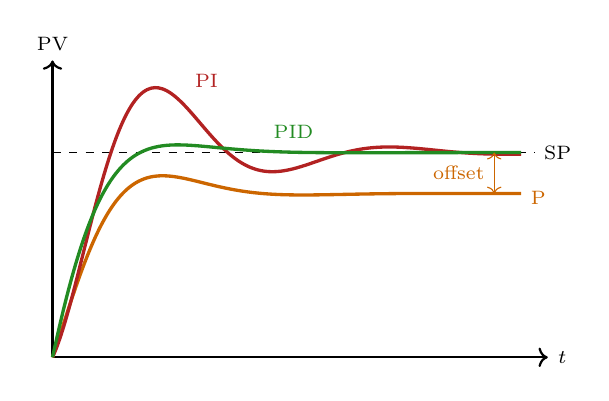
\begin{tikzpicture}[font=\scriptsize, x=0.85cm, y=2.6cm]
					\draw[->, thick] (0,0) -- (7.4,0) node[right] {$t$};
					\draw[->, thick] (0,0) -- (0,1.45) node[above] {PV};
					\draw[dashed] (0,1) -- (7.2,1) node[right] {SP};
					\draw[very thick, cOrange, domain=0:7, samples=120, smooth] plot (\x, {0.8*(1 - exp(-1.2*\x)*cos(deg(1.5*\x)))});
					\draw[very thick, cRed, domain=0:7, samples=120, smooth] plot (\x, {1 - exp(-0.7*\x)*cos(deg(1.8*\x))});
					\draw[very thick, cGreen, domain=0:7, samples=120, smooth] plot (\x, {1 - exp(-1.5*\x)*cos(deg(1.2*\x))});
					\draw[<->, cOrange] (6.6,0.8) -- (6.6,1) node[midway, left] {offset};
					\node[cOrange, right] at (7.0,0.78) {P};
					\node[cRed] at (2.3,1.35) {PI};
					\node[cGreen] at (3.6,1.1) {PID};
				\end{tikzpicture}
			\end{column}
			\begin{column}{0.45\textwidth}
				\renewcommand{\arraystretch}{1.25}
				\centering
				\footnotesize
				\begin{tabular}{@{}lcccc@{}}
					\toprule
					\textbf{Increase} & \textbf{Rise} & \textbf{Over-} & \textbf{Settling} & \textbf{Steady} \\
					& \textbf{time} & \textbf{shoot} & \textbf{time} & \textbf{error} \\
					\midrule
					$K_p$ & $\downarrow$ & $\uparrow$ & small & $\downarrow$ \\
					$K_i$ & $\downarrow$ & $\uparrow$ & $\uparrow$ & \textbf{removed} \\
					$K_d$ & small & $\downarrow$ & $\downarrow$ & none \\
					\bottomrule
				\end{tabular}
				\vspace{0.3cm}
				\begin{itemize}\small
					\item \textbf{P}: fast, but settles \emph{below} SP.
					\item \textbf{PI}: reaches SP, with overshoot.
					\item \textbf{PID}: reaches SP quickly and smoothly.
				\end{itemize}
			\end{column}
		\end{columns}
	\end{frame}

	\begin{frame}{Measuring Performance: The Step Response}
		\begin{columns}[T]
			\begin{column}{0.58\textwidth}
				\centering
				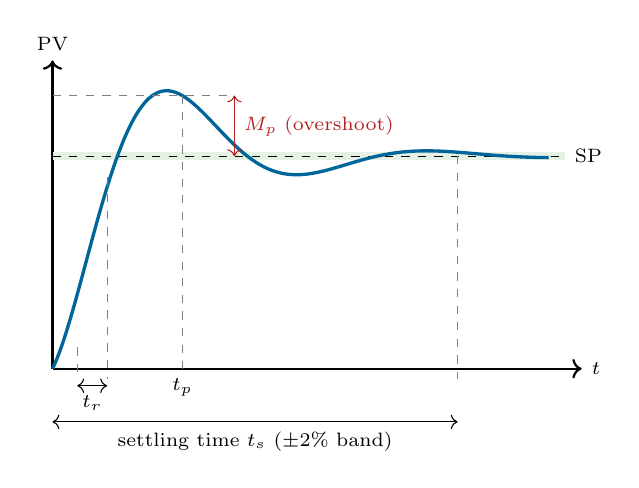
\begin{tikzpicture}[font=\scriptsize, x=1.05cm, y=2.7cm]
					\draw[->, thick] (0,0) -- (6.4,0) node[right] {$t$};
					\draw[->, thick] (0,0) -- (0,1.45) node[above] {PV};
					\fill[cGreen!12] (0,0.98) rectangle (6.2,1.02);
					\draw[dashed] (0,1) -- (6.2,1) node[right] {SP};
					\draw[very thick, cAccent, domain=0:6, samples=150, smooth] plot (\x, {1 - exp(-0.8*\x)*cos(deg(2*\x))});
					% overshoot
					\draw[dashed, gray] (1.571,1.285) -- (1.571,0);
					\draw[<->, cRed] (2.2,1) -- (2.2,1.285) node[midway, right] {$M_p$ (overshoot)};
					\draw[dashed, gray] (0,1.285) -- (2.2,1.285);
					% rise time (10% to 90%)
					\draw[dashed, gray] (0.30,0.1) -- (0.30,-0.05);
					\draw[dashed, gray] (0.66,0.9) -- (0.66,-0.05);
					\draw[<->] (0.30,-0.08) -- (0.66,-0.08) node[midway, below] {$t_r$};
					% settling time (2% band)
					\draw[dashed, gray] (4.9,1) -- (4.9,-0.05);
					\draw[<->] (0,-0.25) -- (4.9,-0.25) node[midway, below] {settling time $t_s$ ($\pm2\%$ band)};
					\node[below] at (1.571,0) {$t_p$};
				\end{tikzpicture}
			\end{column}
			\begin{column}{0.42\textwidth}
				\begin{itemize}\small
					\item \textbf{Rise time $t_r$} --- 10\,\% to 90\,\% of final value.
					\item \textbf{Peak time $t_p$} --- time to the first peak.
					\item \textbf{Overshoot $M_p$} --- $\dfrac{\text{peak} - \text{final}}{\text{final}}\times100\,\%$.
					\item \textbf{Settling time $t_s$} --- stays within $\pm2\,\%$ (or 5\,\%).
					\item \textbf{Steady-state error} --- SP $-$ final PV.
				\end{itemize}
				\vspace{0.1cm}
				\footnotesize Tuning = choosing $K_p, K_i, K_d$ to meet these specifications.
			\end{column}
		\end{columns}
	\end{frame}

	\begin{frame}{Digital (Discrete-Time) PID}
		\begin{block}{Computers sample every $T$ seconds}
			Replace the integral by a \textbf{sum} and the derivative by a \textbf{difference}:
			\[
			u[k] = K_p\,e[k] \;+\; K_i\,T\sum_{j=0}^{k} e[j] \;+\; K_d\,\frac{e[k]-e[k-1]}{T}
			\]
		\end{block}
		\begin{columns}[T]
			\begin{column}{0.5\textwidth}
				\textbf{Example:} $K_p = 2$, $K_i = 0.5$, $K_d = 1$, $T = 1$ s.\\
				Errors so far: $e[0] = 4$, $e[1] = 3$, $e[2] = 1$.
			\end{column}
			\begin{column}{0.5\textwidth}
				\small
				\begin{align*}
					P &= 2\times1 = 2\\
					I &= 0.5\times1\times(4+3+1) = 4\\
					D &= 1\times\tfrac{1-3}{1} = -2\\
					u[2] &= 2 + 4 - 2 = \boxed{4}
				\end{align*}
			\end{column}
		\end{columns}
		\vspace{0.1cm}
		\footnotesize\centering The D term is \emph{negative}: the error is falling fast, so the controller eases off to avoid overshoot.
	\end{frame}

	\begin{frame}[fragile, plain]{}

		\vspace*{0.05cm}

		\begin{columns}[T,onlytextwidth]

			% =========================================================
			% LEFT COLUMN -- PSEUDOCODE
			% =========================================================

			\begin{column}{0.28\textwidth}

				\begin{block}{Pseudocode}
					\scriptsize
					\begin{enumerate}
						\item START
						\item Set $K_p, K_i, K_d$, $T$, SP; \texttt{PV = sum = e\_prev = 0}
						\item \textbf{REPEAT} every $T$
						\begin{itemize}\scriptsize
							\item \texttt{e = SP - PV}
							\item \texttt{sum += e*T}
							\item \texttt{d = (e - e\_prev)/T}
							\item \texttt{u = Kp*e + Ki*sum + Kd*d}
							\item apply \texttt{u}; read \texttt{PV}; \texttt{e\_prev = e}
						\end{itemize}
						\item STOP after 5 s
					\end{enumerate}
				\end{block}

			\end{column}


			% =========================================================
			% MIDDLE COLUMN -- C PROGRAM
			% =========================================================
			\hspace*{0.3cm}
			\begin{column}{0.46\textwidth}

				\begin{block}{C Program (simulated loop)}

\begin{lstlisting}[style=cstyle,numbers=none,basicstyle=\ttfamily\scriptsize]
#include <stdio.h>

int main(void)
{
	float Kp = 2, Ki = 1, Kd = 0.1;
	float T  = 0.1;           /* sample time */
	float sp = 1, pv = 0;     /* SP and PV   */
	float e, e_prev = 0, integ = 0, deriv, u;
	int k;

	for (k = 1; k <= 50; k++) {
		e      = sp - pv;
		integ += e * T;
		deriv  = (e - e_prev) / T;
		u      = Kp*e + Ki*integ + Kd*deriv;
		pv    += T * (u - pv);   /* plant */
		e_prev = e;
		if (k % 10 == 0)
			printf("t=%.1f s  PV=%.3f\n", k*T, pv);
	}
	return 0;
}
\end{lstlisting}

				\end{block}

			\end{column}


			% =========================================================
			% RIGHT COLUMN -- FLOWCHART
			% =========================================================

			\begin{column}{0.26\textwidth}

				\begin{tikzpicture}[
					remember picture,
					overlay
					]

					\node at ([xshift=62mm,yshift=8mm]current page.center)
					{
						\begin{tikzpicture}[
							scale=0.6,
							transform shape,
							>=Stealth,
							every node/.style={
								font=\small,
								align=center
							},
							startstop/.style={
								ellipse,
								draw=black,
								line width=0.8pt,
								minimum width=22mm,
								minimum height=8mm,
								text=black,
								fill=gray!15
							},
							process/.style={
								rectangle,
								draw=black,
								line width=0.8pt,
								minimum width=30mm,
								minimum height=9mm,
								text=black,
								fill=orange!15
							},
							decision/.style={
								diamond,
								draw=black,
								line width=0.8pt,
								aspect=2,
								minimum width=25mm,
								minimum height=15mm,
								inner sep=1pt,
								text=black,
								font=\scriptsize,
								fill=green!15
							},
							flow/.style={
								->,
								line width=0.8pt
							}
							]

							% -------------------------------------------------
							% Nodes
							% -------------------------------------------------

							\node[startstop] (start) {START};

							\node[process, below=6mm of start, fill=blue!10] (init)
							{Initialise gains,\\ SP, PV, sum};

							\node[process, below=6mm of init] (err)
							{$e = \text{SP} - \text{PV}$};

							\node[process, below=6mm of err] (pid)
							{$u = K_p e + K_i\!\sum\! e\,T$\\ $+\,K_d\,\Delta e/T$};

							\node[process, below=6mm of pid] (plant)
							{apply $u$,\\ read new PV};

							\node[decision, below=8mm of plant] (decision)
							{$k < 50$?};

							\node[startstop, below=8mm of decision] (stop)
							{STOP};

							% -------------------------------------------------
							% Main vertical flow
							% -------------------------------------------------

							\draw[flow] (start) -- (init);
							\draw[flow] (init) -- (err);
							\draw[flow] (err) -- (pid);
							\draw[flow] (pid) -- (plant);
							\draw[flow] (plant) -- (decision);

							% -------------------------------------------------
							% YES branch: loop back
							% -------------------------------------------------

							\draw[flow]
							(decision.east)
							-- ++(12mm,0)
							|- (err.east);

							\node[
							font=\scriptsize,
							text=green!40!black
							] at ($(decision.east)+(5mm,3mm)$)
							{YES};

							% -------------------------------------------------
							% NO branch
							% -------------------------------------------------

							\draw[flow]
							(decision.south)
							-- node[
							right=1mm,
							font=\scriptsize,
							text=red!70!black
							] {NO}
							(stop.north);

						\end{tikzpicture}
					};

				\end{tikzpicture}

			\end{column}

		\end{columns}

		\begin{tikzpicture}[remember picture,overlay]

			\node[
			anchor=south west,
			draw,
			rounded corners=2pt,
			fill=white,
			text width=3.6cm,
			align=left,
			inner sep=5pt
			] at ([xshift=2mm,yshift=3mm]current page.south west)
			{
				\textbf{Program Output}\\[3pt]
				\ttfamily\scriptsize
				t=1.0 s\ \ PV=0.772\\
				t=2.0 s\ \ PV=0.868\\
				t=3.0 s\ \ PV=0.911\\
				t=4.0 s\ \ PV=0.939\\
				t=5.0 s\ \ PV=0.959
			};

		\end{tikzpicture}

	\end{frame}

	% =================================================================
	\section{Tuning of PID Controllers}
	% =================================================================
	\begin{frame}{What is Controller Tuning?}
		\begin{block}{Tuning}
			Choosing the controller parameters ($K_p$, $T_i$, $T_d$) so that the loop is \textbf{stable}, \textbf{fast} and has \textbf{acceptable overshoot} for \emph{this particular} process.
		\end{block}
		\vspace{0.05cm}
		\renewcommand{\arraystretch}{1.12}
		\centering
		\footnotesize
		\begin{tabular}{@{}>{\raggedright}p{3.4cm}>{\raggedright}p{5.6cm}>{\raggedright\arraybackslash}p{3.6cm}@{}}
			\toprule
			\textbf{Method} & \textbf{Idea} & \textbf{Needs} \\
			\midrule
			Manual (trial \& error) & adjust P, then I, then D while watching the trend & experience, time \\
			Ziegler--Nichols \emph{closed loop} & push loop to sustained oscillation, use formulas & ultimate gain $K_u$, period $P_u$ \\
			Ziegler--Nichols \emph{open loop} & step test of the process (reaction curve) & delay $L$, time constant $T$ \\
			Cohen--Coon, IMC, Lambda & model-based refinements & process model \\
			Auto-tuning & controller runs its own test (relay method) & modern PLC / controller \\
			\bottomrule
		\end{tabular}
	\end{frame}

	\begin{frame}{Manual (Trial-and-Error) Tuning}
		\begin{block}{Before you start}
			Put the controller in \textbf{AUTO} with $T_i = \infty$ (I off) and $T_d = 0$ (D off). Make small setpoint steps and watch the PV trend.
		\end{block}
		\centering
		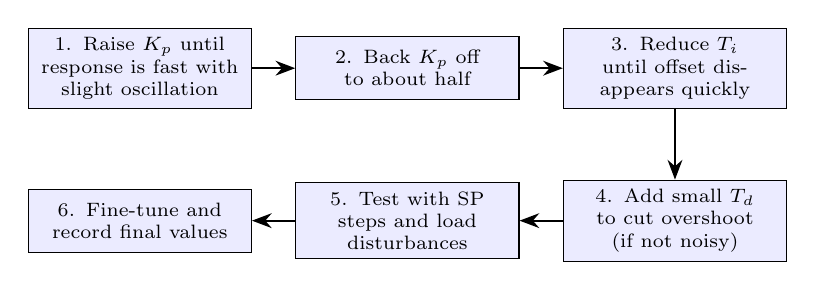
\begin{tikzpicture}[every node/.style={font=\scriptsize}, node distance=0.55cm, process/.append style={minimum width=2.6cm, text width=2.6cm}]
			\node[process] (p1){1. Raise $K_p$ until response is fast with slight oscillation};
			\node[process, right=of p1] (p2){2. Back $K_p$ off to about half};
			\node[process, right=of p2] (p3){3. Reduce $T_i$ until offset disappears quickly};
			\node[process, below=0.9cm of p3] (p4){4. Add small $T_d$ to cut overshoot (if not noisy)};
			\node[process, left=of p4] (p5){5. Test with SP steps and load disturbances};
			\node[process, left=of p5] (p6){6. Fine-tune and record final values};
			\draw[flowarrow](p1)--(p2); \draw[flowarrow](p2)--(p3);
			\draw[flowarrow](p3)--(p4); \draw[flowarrow](p4)--(p5); \draw[flowarrow](p5)--(p6);
		\end{tikzpicture}
		\vspace{0.15cm}
		\begin{itemize}\small
			\item Change \textbf{one} parameter at a time, by a factor of about 2.
			\item Many real loops (flow, level, pressure) work well as \textbf{PI} only.
		\end{itemize}
	\end{frame}

	\begin{frame}{Ziegler--Nichols Closed-Loop (Ultimate Gain) Method}
		\begin{columns}[T]
			\begin{column}{0.5\textwidth}
				\begin{enumerate}\small
					\item Use \textbf{P-only} control ($T_i = \infty$, $T_d = 0$).
					\item Increase $K_p$ slowly until the PV oscillates with \textbf{constant amplitude}.
					\item Record that gain $K_u$ (\emph{ultimate gain}) and the oscillation period $P_u$.
					\item Read the settings from the table.
				\end{enumerate}
				\vspace{0.1cm}
				\centering
				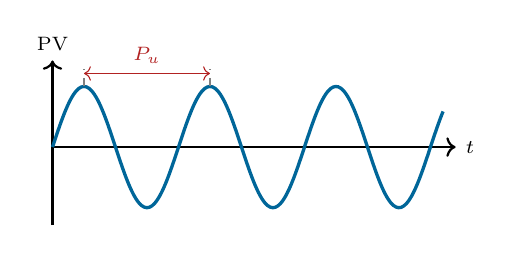
\begin{tikzpicture}[font=\scriptsize, x=0.8cm, y=1.1cm]
					\draw[->, thick] (0,0) -- (6.4,0) node[right] {$t$};
					\draw[->, thick] (0,-0.9) -- (0,1.0) node[above] {PV};
					\draw[very thick, cAccent, domain=0:6.2, samples=150, smooth] plot (\x, {0.7*sin(deg(2*pi*\x/2))});
					\draw[<->, cRed] (0.5,0.85) -- (2.5,0.85) node[midway, above] {$P_u$};
					\draw[dashed, gray] (0.5,0.7) -- (0.5,0.9);
					\draw[dashed, gray] (2.5,0.7) -- (2.5,0.9);
				\end{tikzpicture}
			\end{column}
			\begin{column}{0.5\textwidth}
				\renewcommand{\arraystretch}{1.4}
				\centering
				\begin{tabular}{@{}lccc@{}}
					\toprule
					\textbf{Type} & $\bm{K_p}$ & $\bm{T_i}$ & $\bm{T_d}$ \\
					\midrule
					P   & $0.5\,K_u$  & $\infty$       & $0$ \\
					PI  & $0.45\,K_u$ & $P_u/1.2$      & $0$ \\
					PID & $0.6\,K_u$  & $P_u/2$        & $P_u/8$ \\
					\bottomrule
				\end{tabular}
				\vspace{0.3cm}
				\begin{block}{Caution}
					\small Driving a real plant to the edge of instability can be unsafe --- the \emph{relay auto-tune} method finds $K_u$, $P_u$ with a small, controlled oscillation.
				\end{block}
			\end{column}
		\end{columns}
	\end{frame}

	\begin{frame}{Ziegler--Nichols Open-Loop (Process Reaction Curve) Method}
		\begin{columns}[T]
			\begin{column}{0.5\textwidth}
				\small
				With the controller in \textbf{MANUAL}, make a step change in the output and record the PV. Draw the tangent at the steepest point:
				\centering
				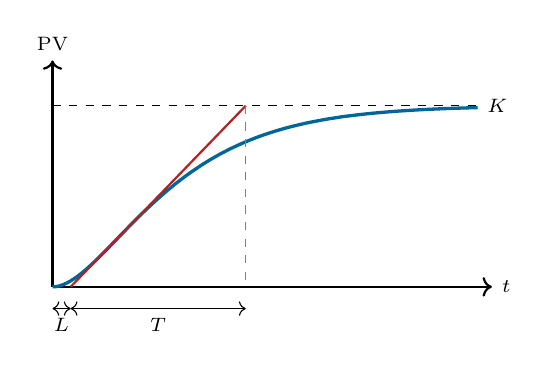
\begin{tikzpicture}[font=\scriptsize, x=0.9cm, y=2.3cm]
					\draw[->, thick] (0,0) -- (6.2,0) node[right] {$t$};
					\draw[->, thick] (0,0) -- (0,1.25) node[above] {PV};
					\draw[dashed] (0,1) -- (6,1) node[right] {$K$};
					\draw[very thick, cAccent, domain=0:6, samples=120, smooth] plot (\x, {1 - (1 + 1.1*\x)*exp(-1.1*\x)});
					% tangent at inflection x = 1/1.1 = 0.909
					\draw[thick, cRed] (0.256,0) -- (2.727,1);
					\draw[dashed, gray] (2.727,1) -- (2.727,0);
					\draw[<->] (0,-0.12) -- (0.256,-0.12) node[midway, below] {$L$};
					\draw[<->] (0.256,-0.12) -- (2.727,-0.12) node[midway, below] {$T$};
				\end{tikzpicture}

				\footnotesize $L$ = dead time,\; $T$ = time constant,\; $K$ = process gain ($\Delta$PV/$\Delta$CO).
			\end{column}
			\begin{column}{0.5\textwidth}
				\renewcommand{\arraystretch}{1.4}
				\centering
				\begin{tabular}{@{}lccc@{}}
					\toprule
					\textbf{Type} & $\bm{K_p}$ & $\bm{T_i}$ & $\bm{T_d}$ \\
					\midrule
					P   & $T/(KL)$      & $\infty$  & $0$ \\
					PI  & $0.9\,T/(KL)$ & $3.33\,L$ & $0$ \\
					PID & $1.2\,T/(KL)$ & $2\,L$    & $0.5\,L$ \\
					\bottomrule
				\end{tabular}
				\vspace{0.3cm}

				\small Works for self-regulating processes that look like ``first order + dead time'' (temperature, pressure).
			\end{column}
		\end{columns}
	\end{frame}

	\begin{frame}{Tuning: Worked Examples}
		\begin{columns}[T]
			\begin{column}{0.5\textwidth}
				\begin{block}{Closed-loop method}
					\small A P-only test gives sustained oscillation at $K_u = 10$ with period $P_u = 2$ s. Find PID settings.
				\end{block}
				\small
				\begin{align*}
					K_p &= 0.6\times10 = \boxed{6}\\
					T_i &= 2/2 = 1\ \text{s} \;\Rightarrow\; K_i = K_p/T_i = 6\ \text{s}^{-1}\\
					T_d &= 2/8 = 0.25\ \text{s} \;\Rightarrow\; K_d = K_p T_d = 1.5\ \text{s}
				\end{align*}
			\end{column}
			\begin{column}{0.5\textwidth}
				\begin{block}{Open-loop method}
					\small A step test on a heater gives $K = 1$, dead time $L = 2$ s, time constant $T = 10$ s. Find PI and PID settings.
				\end{block}
				\small
				\begin{align*}
					\text{PI:}\quad K_p &= 0.9\times\tfrac{10}{1\times2} = \boxed{4.5},\quad T_i = 6.67\ \text{s}\\
					\text{PID:}\quad K_p &= 1.2\times\tfrac{10}{2} = \boxed{6}\\
					T_i &= 2\times2 = 4\ \text{s},\quad T_d = 0.5\times2 = 1\ \text{s}
				\end{align*}
			\end{column}
		\end{columns}
		\vspace{0.2cm}
		\footnotesize\centering Ziegler--Nichols values give a quick, ``aggressive'' response ($\approx$25\,\% overshoot) --- treat them as a \textbf{starting point} and fine-tune.
	\end{frame}

	\begin{frame}{Practical Issues in Real PID Loops}
		\begin{columns}[T]
			\begin{column}{0.5\textwidth}
				\begin{block}{Integral windup}
					\small When the valve is already 100\,\% open, the integral keeps growing; when the error reverses, it takes a long time to ``unwind'' $\rightarrow$ big overshoot.\\
					\textbf{Fix:} clamp the integral (anti-windup).
				\end{block}
				\begin{block}{Derivative kick}
					\small A sudden SP step makes $de/dt$ huge $\rightarrow$ output spike.\\
					\textbf{Fix:} take the derivative of the \emph{PV}, not the error.
				\end{block}
			\end{column}
			\begin{column}{0.5\textwidth}
				\begin{block}{Measurement noise}
					\small D action amplifies noise.\\
					\textbf{Fix:} filter the PV, or use PI only.
				\end{block}
				\begin{block}{Bumpless transfer}
					\small Switching MANUAL $\leftrightarrow$ AUTO must not make the output jump.\\
					\textbf{Fix:} initialise the integral to the current output.
				\end{block}
				\begin{block}{Controller action}
					\small \textbf{Reverse} (heating: PV $\uparrow$ $\Rightarrow$ output $\downarrow$) or \textbf{direct} (cooling). Wrong choice = runaway loop!
				\end{block}
			\end{column}
		\end{columns}
	\end{frame}

	\begin{frame}{Summary \& What Comes Next}
		\begin{columns}[T]
			\begin{column}{0.5\textwidth}
				\begin{block}{Concept}
					\begin{itemize}\small
						\item Industrial processes: continuous, batch, discrete; automation levels.
						\item Control loop elements: sensor, controller, final control element.
						\item Pneumatic, hydraulic \& electrical systems; PLC and ladder logic.
						\item Valves (directional, pressure, flow, control) and actuators.
						\item Stepper motors: types, step angle, drive sequences.
						\item PID control and its tuning (manual, Ziegler--Nichols).
					\end{itemize}
				\end{block}
			\end{column}
			\begin{column}{0.5\textwidth}
				\begin{block}{Practice makes perfect}
					\begin{itemize}\small
						\item Re-work every numerical example yourself.
						\item Draw the valve symbols from memory.
						\item Run the PID C program; change $K_p, K_i, K_d$ and watch the PV.
					\end{itemize}
				\end{block}
				\begin{block}{Coming up}
					\small PLC programming, sensors \& transducers, and marine automation systems.
				\end{block}
			\end{column}
		\end{columns}
	\end{frame}

	%------------------------------------------------
	\begin{frame}
		\centering
		\Huge Thank You
		\vspace{0.5cm}

		\normalsize Questions?
	\end{frame}

	%------------------------------------------------

\end{document}
